%!TEX root = project.tex

\chapter*{About this project}
% assuming past tense as this report is talking about the completed project
\paragraph{Abstract}
%A brief description of what the project is, in about two-hundred and fifty words.

% leave technical jargon out of it
This project sets out to create a food ordering system for a local company. 
The systems primary components are a mobile application that the user interacts with and a web application that the staff interact with.

The need for such a system stems from two problems, firstly the issue of rush hour times during business hours where there is a vast number of customers to service, and secondly to bring more presence and promotion to the business, as they are finding it hard to reach out to their current customer base and would be customers.

% Mobile app
We aim to solve the first problem by having a system in which customers can pre-order sandwiches and other products via a mobile application.
Users will be able to top up their account, order products, pick a collection time, and view their balance, products and past order history.

The second problem will be solved by implementing push notifications into the application so that the company can let customers know about menus, events and various other updates. Another way to increase promotion and presence is by having various information about the company on the application; for instance: opening times, contact details and general information. 

% web app
All of the information on the web application can be updated; this includes the menus, opening times, user and staff details, and much more. 
This information is reflected in the web application.
Interactions from within the mobile application including: topping up, logging in, registration and ordering go through the web application.

% conclusion
We plan to create a cohesive, thoughtfully designed, robust system that solves these two problems.
\pagebreak


\paragraph{Authors}
%Explain here who the authors are.
This project was created by two fourth year software development students: Ronan Connolly \& Vladislav Marisevs, as part of our Bachelors of Science honours degree in Software Development.
\\

Ronan was in charge of creating all aspects of the user facing mobile app. 
Vladislav was in charge of creating all aspects of the staff facing web app.
\\

We spent most of our shared time coming up with the overall architecture we would implement, and an interface to be used between mobile and web app for transfer of data.
\pagebreak

\paragraph{Acknowledgements}
We would like to acknowledge and thank our supervisor Dr John Healy for all the time and effort he has put into helping us throughout this project, he gave us a good structure and set milestones for us in order to keep on top of things.
\\

We'd also like to thank the GMIT Catering Company staff for the time spent meeting with us in order to continuously improve and adapt the project.

\chapter{Introduction}	% 3-5 pages
%% CONTEXT
% basic idea
We set out to create a food ordering system for the GMIT Catering Company (known henceforth as the company).
The basic structure is a mobile application (henceforth known as mobile app) for the Android and iOS systems that the user interacts with, and a server (henceforth known as web app) that the staff can log into in order to view transactions, user details and to update the mobile app.

% reason #1
The reason such a system is needed is that queues during peak times tend to be enormous and currently it's hard to service all the customers.

% reason #2
Another reason is to encourage customers to get into a habit of repeat ordering, if it is an easy process then it should increase purchases.

% reason #3
Lastly, the company wants to increase presence and promotion in the college, in order to achieve this end we have implemented push notifications where staff can send a notification to all users. On top of this the mobile application itself serves as a promotional device, containing details of various aspects of the company.
\\

%% OBJECTIVES
% actual system:
In order to develop this system we required to connect different platforms together and let them communicate. We were using Ionic Framework for creating cross mobile application that would talk to Zend Framework 2 which will act as administration website and API (Application Programming Interface) for controlling data transfer between MySQL database and mobile program.
\\

% mobile app features
The components contained within the mobile app include pages for login, registration, about the company and user details There is also a way to top up and order sandwiches.
A huge emphasis is put on design for this project, using the companies colour theme and creating a nice icon.
% tech
This mobile app was created using the Ionic Framework which is programmed primarily using the AngularJS framework.
% Ionic part:
It's a cross platform mobile application that will authenticate users using their credentials. This option will allow us to create an account wallet, identify a person and their order history. The mobile app design uses native phone features and user interface components to let user operate without any special training.
\\

% web app features
The components contained within the web app include many pages such as the login system, orders, stock, user details, vouchers(for adding credit to your account), settings(collection and opening times) and accounts(staff) pages.
% Zend part:
This web app is a administration website which allows user to configure and manage the whole system. Users can change opening, closing and food collection times. In order to access these settings users should authenticate him self and then will be able to nominate new administration members. This website also allows to view list of orders, customers and track their history.  
%Some of these routes acts as connections that informs mobile application about changes or receives 
\\

%tech
This web app was created in PHP using Zend Framework 2.
% reflection in app
Most of the information on the web app is reflected on the mobile app.

% connect the apps
The two applications talk to each other via JSON over HTTP Get and Post requests. 

% conclusion
We set out to create a well thought out, carefully designed, robust food ordering system using modern technologies.
This project could be extended in the future to be used 
\\

% mention agile
We used an agile structure where we had certain components we needed complete by specific dates.
% mention meetings
We had various meetings each month with our supervisor and several members of the company.

%% CHAPTER SUMMARIES
\section{Chapter Summaries}
Here is a summary of all the chapters in this project report.

\subsection*{Context}
Here we talk about how the project came about, what the initial ideas, goals and objectives were.
We'll also talk about the main components of our project, how we chose them, the alternatives we tried out and a basic overview of the usage of our food ordering system.

\subsection*{Methodology}
An insight into how we began the project, the research, our technology and design choices, our thought process and how we went about allocating tasks and organising meetings.

We'll also talk about the objectives we set out to accomplish and how we went about completing them.

\subsection*{Technology Review}
Here we talk about all the technologies that we have mentioned in this report and any others that we may have used in completing the project.

\subsection*{System Design}
An overview of the project architecture, including lots of diagrams and screen shots.

\subsection*{System Evaluation}
An evaluation of our various project components, including how we tested our system for robustness and performance.
We talk about the outcomes that were achieved in relation to what are goals were, how far we strayed from our goals and some issues we came up against.
Any limitations or opportunities we encountered in our approach and in the technologies we chose.

\subsection*{Conclusion}
A broad overview of our development work-flow, from our thought processes, meetings, technology choices to our issues,problems and perceptions of the project as a whole.
We'll touch on our overall experience and what we would have done differently.

% - List the resources URL(GitHub address for the project and provide a brief list of the main elements at the URL)
\section{GitHub Links}
The web and mobile app repositories are private so you must ask to be added as a collaborator in order to view them.
Each section below has a clickable heading and contains a link to the respective GitHub repository.

\subsection*{\href{https://github.com/GMIT-Catering}{GMIT Catering Organisation}}
This GitHub organisation was created to host all repositories related to this project \cite{github_org}.
These projects will be maintained here or forked here on completion.

\subsection*{\href{http://gmit-catering.github.io/final-year-project-template/}{Gist ReadMe}}
This contains basic instructions for using each component of the project \cite{gh_gist_readme}.

\subsection*{\href{https://github.com/VMarisevs/CanteenOrderSystem}{Web App}}
The food ordering web app \cite{gh_web_app}.

\subsection*{\href{https://github.com/RonanC/gmit-catering}{Mobile App}}
The Ionic mobile application \cite{gh_mobile_app}.

\subsection*{\href{https://github.com/RonanC/gmit-catering-test-server}{Test Server}}
The test server that we used initially to test the mobile app \cite{gh_test_server}.
This received requests and sent back mock data that imitated the real server.

\subsection*{\href{https://github.com/RonanC/gmitcat-push}{Push Web App}}
This web application is using the MEAN stack technologies \cite{gh_push_webapp}.
It is hosted on Heroku and is used to save user details.
Administrators can log in and send push notification messages to registered users.

\subsection*{Project Report}
The project report that you are currently reading \cite{gh_project_report}.

\chapter{Context}	% 3-5 pages

\begin{itemize}
\item Our project consists of creating a food ordering system for the GMIT Catering Company.
\item Our basic objectives were to create a mobile and web application to deal with the above item.
\end{itemize}

% - Briefly list each chapter/section and provide 1-2 line description of what each section contains
Below we will:
\begin{itemize}
\item explain the various components of our project.
\end{itemize}

\section{System Administration and Management Web Application}

The PHP is widely used as a popular server side language and great number of open source software and company’s web sites use PHP since it can enable high software productivity\cite{PHP_Usage}.

IBM Research group from Tokyo Research Laboratory reports that PHP as a web service engine performs competitively with Axis2 Java for web services involving small payloads, and greatly outperforms it for larger payloads by 5-17 times. As the authors expected, Axis2 C performs best, but the experimental results demonstrate that PHP performance is closer to Axis2 C with larger payloads\cite{Web_Service_Engines_in_PHP_Java_C}.

In order to develop a secure web application, Zend Framework 2 was chosen as base of this project. From the various types of PHP frameworks it was designed by Zend Technologies Ltd, who also developed PHP license. Appendix \ref{appendix:LiteratureReviewZF} describes cross-site scripting attacks and how to prevent them using Zend Framework.
%% to be continue 


\section{Mobile App}
The mobile application is created using bleeding edge technologies such as the Ionic framework, which utilizes the AngularMVW framework, which in turn is programmed using JavaScript. HTML and CSS were also heavily utilized.
\\

Initially I had no idea about JavaScript, web development or cross platform development. I spent much time studying JavaScript, Angular, Ionic, and the MEAN Stack (MongoDB, ExpressJS, AngularJS, and NodeJS). I then spent a lot fo time trying out various cross platform development frameworks.
\\

I will speak more in detail about these technologies in the technology review chapter.
\\

Some of the features of the mobile application are:
\begin{itemize}
\item Login
\item Sign-up
\item Password Reset
\item Food Ordering
\item About Information
\item Account Information
\item Password change
\item User History
\item Topping up
\end{itemize}
I will go through these features in detail in the system design chapter.

\subsection{Cross Platform Frameworks}
I first tried out Cordova \cite{cordova}, which I found had the capabilities to do pretty much anything, but the community and framework is very sparse, it's hard to get anything up \& running, and the styling's are horrid.
\\

Next I tried out JQueryMobile \cite{jquery_mobile} which had better styling but again I came across many issues.
\\

Finally I came across the Ionic Framework \cite{ionic} which uses Cordova underneath. This framework has a huge community of developers, it has the support of Google, Microsoft and many other large companies. They closely work with the Angular team at Google and the TypeScript team at Microsoft. 
They have a 24/7 group chat system set up with various sub rooms. 
They have amazing documentation, regular blog posts, quick response to questions on the blog, forums and chat. 
With Ionic you get:
\begin{itemize}
\item All the capabilities of Cordova, which allows you to access the Mobiles native APIs easily
\item A slick native UI experience. The app changes design depending on the platform it's running on
\item Extensive tooling. Starting an app, templates, app store image creation, logo creator, etc
\item Rapid development cycle, there are constant updates (which can cause issues, but is usually great)
\end{itemize}

\subsection{Tooling}
Once I decided on using the Ionic framework I spent my time completing various JavaScript, Angular and Ionic tutorials. This was a steep learning curve as there is so much tooling for all the JavaScript frameworks.
I installed NodeJS in order to use NPM (Node Package Manager) in order install Ionic. 

Then Ionic came with it's own tools for various tasks, including SASS for programmatic CSS, Bower (Like NPM or Maven) for adding in new components, Grunt for running tasks (like Ant) and some others like Gulp (similar again to NPM).

Each of these tools takes time to learn. I read documentation and completed at least one tutorial for each.

\section{Push Server}
In order to facilitate push notifications I needed to get their device token and save it in a database.
I created a controller in the mobile application, once the app starts it gets the device token along with some other information and sends it to the push server.

The push server is always listening for incoming requests, once it receives one it evaluates it, adds a timestamp and saves the user object (JSON) to a CouchDB server (Using IBM's Cloudant Web Server).

The push server is a MEAN Stack, Yeoman scafolded project that uses NodeJS as the environment, Express as the Web Framework and Angular as the MVC (Model View Controller) framework in order to build the web application.
\linebreak

The reasons we chose to have the push notification server separate is that:
\begin{itemize}
\item We did not realise we needed to save the device tokens initially and to implement this new table into the SQL schema is a big effort
\item We wanted to try out a MEAN Stack application
\item We felt there was no big dissadvantage on having the push server seperate
\item The mobile app is so tightly integrated with the push server (everything is written in JavaScript), that it made creating the web application extremely simple
\item The GMIT Catering company may assign the task of push notifications to somebody that they do not wish to have access to the food ordering system, such as a social media expert. 
\end{itemize}

Users can:
\begin{itemize}
\item Login/Logout via username and password
\item View how many devices are registered for push notifications
\item View previously sent push notifications
\item Send new push notifications, and see if they were sent successfully.
\end{itemize}


\chapter{Methodology}	% 1-2 pages
% Describe the way you went about your project:
\begin{comment}
\begin{itemize}
	\item We used an Agile / incremental and iterative approach to development. 
	\item There were plenty of meeting and planning with our supervisor and the companies manager.
	\item We did user testing on the app, and constantly made sure all the routes were working.
	\item We designed a RESTful style route interface. This let us work on our own components without the web and mobile app waiting for each other.
	\item We used GitHub during the development process, tracking tasks via the Github Issue tracker.
	\item We tested out various technologies at each step of the way and discussed why we were choosing each one.
\end{itemize}
\end{comment}
When we began this project we knew we had to split it up into sections and allocate parts to one another.  
Since Ronan had worked on many mobile applications before and Vlad had created various web applications in conjunction with large databases we decided Ronan would take on the mobile side and Vlad the web app \& database.
\\

We have already spoken in the Introduction why we chose the technologies we chose so here we will focus on our implementation of these technologies.

\section{Direction}
%How we went about our project
% agile
We took some inspiration from the "Manifesto for Agile Software Development" and tried to implement some of the aspects.
As well as this we looked into SCRUM and RAD.

We used the GitHub issue tracker to work through tasks, flag bugs and add enhancement requests.
We found that the regular meetings and feedback were great for tweaking design but it held us back in many respects.
There were times when we needed to overhaul the design that took much time, especially when it involved changing the database scheme (SQL does not like this).

\subsection{Interface}
Due the fact that the mobile app relied on the server which would not be complete for some time, we needed to come up with a common interface we could both program towards.
This idea was inspired by Edsgar Dijkstra:
\begin{quote}
	% \blindtext
	\itshape He worked closely with Bram J. Loopstra and Carel S. Scholten, who had been hired to build a computer. Their mode of interaction remains a model of disciplined engineering: They would first decide upon the interface between the hardware and the software, by writing a programming manual. Then the hardware designers would have to be faithful to their part of the contract, while Dijkstra, the programmer, would write software for the nonexistent machine. Two of the lessons he learned from this experience were the importance of clear documentation, and that program debugging can be largely avoided through careful design.
	\hfill 
	\\
	- The University of Texas at Austin - The General Faculty \cite{dijkstra_interface}
	% \par
	% \begingroup
	% \leftskip4em
	% \rightskip\leftskip
	% \blindtext
	% \par
	% \endgroup
	% \blindtext
\end{quote}

We decided to create a RESTful API on your web server, to which the mobile application could query.
In order to test the mobile application in the mean time, we created a test server that would receive a request and return mock data.
We could then switch between the real and test server with one line of code change.
This also helped us find bugs, if the test server worked and the real server did not, then we knew there was an error on the real server.
This test server was written with the MEAN stack of technologies (except without MongoDB).
\\

MEAN:
\begin{itemize}
\item MongoDB
\item ExpressJS
\item AngularJS
\item NodeJS
\end{itemize}

The reason we chose this is that for RAD (Rapid Application Development) the MEAN stack is very easy to use.
Especially since the Ionic framework is already using AngularJS and shares many of the same tools including the NPM (Node Package Manager).
\\
\pagebreak
Here is a piece of code from the test server.
This code is for logging in:
\begin{minted}[%
breaklines,
mathescape,
linenos,
numbersep=5pt,
frame=single,
numbersep=5pt,
xleftmargin=0pt,
]{js}
// login
app.get('/verifyuser/:customerLg/:customerPW', function(req, res){
    var result = {
        "customer_id":"11E4E6370B663F0D81B9EC9A743CC2AE",
        "customer_name":"Regina",
        "customer_surname":"Walsh",
        "customer_cash":"10.20",
        "customer_mobile":"0853243435"};

    res.contentType('application/json');
    res.send(JSON.stringify(result));
});
\end{minted}
\begin{comment}
This is for minted
[%
breaklines,
mathescape,
linenos,
numbersep=5pt,
frame=single,
numbersep=5pt,
xleftmargin=0pt,
]
\end{comment}
I hosted this test server on Heroku \cite{heroku}.
Heroku hosts projects as git projects, so you just need to add a config file and push to your heroku repository.
Once complete your project is running live in the wild.
Again this is another nudge towards RAD.

\subsection{Bleeding Edge Technologies}
We wanted to use bleeding edge technologies in our project, since this is our final year project we wanted to use it as a chance to research some novel technologies and see what is possible, while at the same time creating a robust system with a well thought out design.
\\
While cutting edge refers to the newest technology, it also infers that the technology has gone through the wars and is battle-tested (to a degree where it can be considered for review). 
\\
Bleeding edge is different in the sense that it is so new, that we don't even know if it will be around for very long, or whether the current merit it is receiving is worthy or is caused by the hype at the time.
\\
Bleeding edge technologies are all around, especially right now within the web development community, it seems there is a new framework or API that you \textbf{must} know every other day.
\\
We chose some bleeding edge technologies that we felt would stand the test of time and make it into the \textit{cutting edge} stage.
Here is a list of some of these technologies:
\begin{itemize}
	\item AngularJS
	\item Ionic Framework
	\item NodeJs \& ExpressJS
	\item Heroku
\end{itemize}

AngularJS is owned by Google, and Microsoft have started working with them.
This is a good indication of a solid technology, along with all the statistics on it's performance and adoption.
\\
The Ionic Framework has grown to be the most popular cross platform framework.
They work closely with the AngularJS team, and they were even presenting at the Microsoft Build 2016 conference, which is interesting since Microsoft just bought Xamarin which would be considered a competitor.
\\
NodeJS and ExpressJS were used for the test server and the push web application. 
These are still in there infancy but the Node Package Manager (NPM) has in a few short years grown to be the most popular package management system out there.
\\
We did not know any of these technologies coming into this project, so the learning curve was very high and it tested us throughout the development life-cycle. Many things were learned from proper planning, emailing, documenting progress, using Git properly, setting milestones, dealing with clients and the time spent learning/studying technologies compared to actually implementing them.
\\

Here are some graphs showing the growth trend among various package managers \cite{module_counts}:
\begin{figure}[H] 
	\center{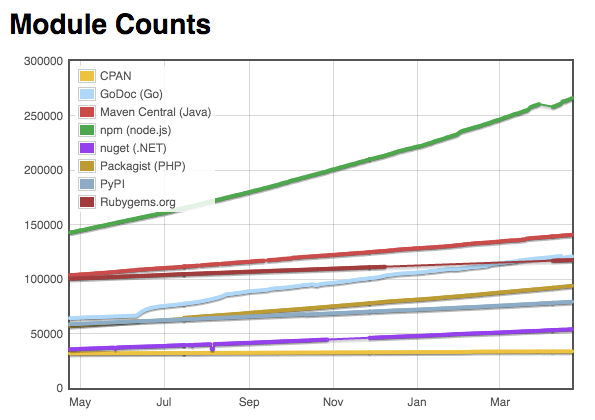
\includegraphics[width=0.75\linewidth]{img/module_counts_year}}
	\caption{Module Count Growth in the last Year }
	\label{fig:speciation}
\end{figure}
We can see here that NPM is the clear winner.
This is due to the fact that the community is so alive, connected and are really into open source software development.

In this graph we can see exponential growth from NPM:
\begin{figure}[H] 
	\center{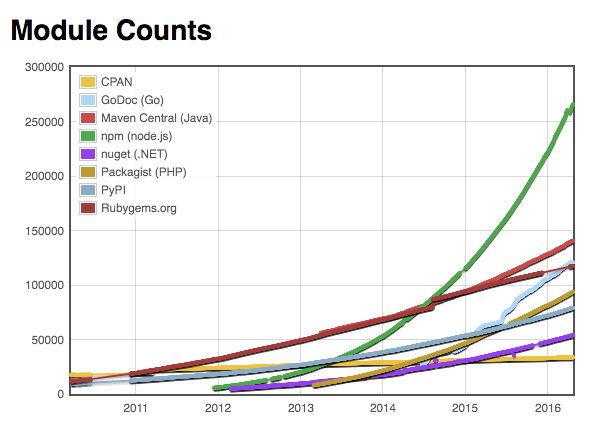
\includegraphics[width=0.75\linewidth]{img/module_counts_alltime}}
	\caption{Module Count Growth All-time }
	\label{fig:speciation}
\end{figure}

Server Providers that use the git \cite{git} technology to allow users to manage their servers are becoming increasingly more popular as time goes on.
Examples of this our companies like Heroku.
This makes it very easy to maintain, manage and utilize a RAD type of development.

\section{Agility}
% Agile / incremental and iterative approach to development. Planning, meetings.
We wanted to be flexible in our approach since most of the aspects involved from meetings, planning, project development and the technologies were new to use. Agile suited us well.

\subsection{Agile}
We decided that we wanted to go through this project in a modern way so we looked into the \textit{"Manifesto for Agile Software Development"} \cite{manifesto_for_agile}:
\begin{figure}[H] 
	\center{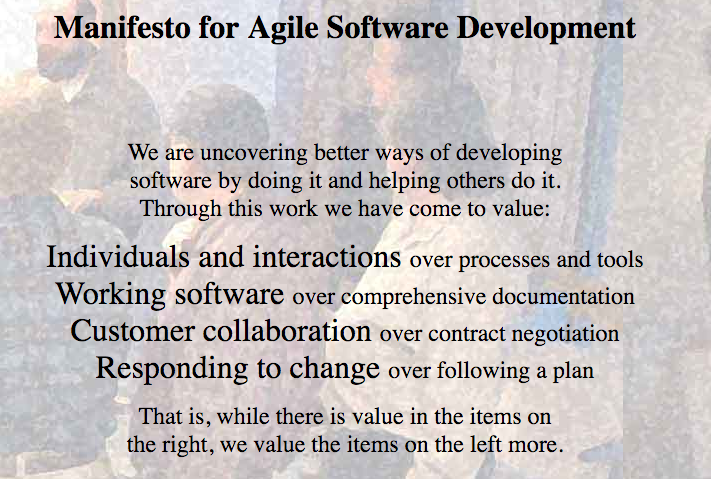
\includegraphics[width=1.0\linewidth]{img/manifesto_for_agile}}
	\caption{Manifesto for Agile Software Development}
	\label{fig:speciation}
\end{figure}
With these ideas behind us (and some more taken from SCRUM and RAD) we worked to:
\begin{itemize}
	\item Have regular meetings with our client
	\item Constantly take feedback on board
	\item Change designs throughout development where possible
	\item Break down tasks into their constituents and work through them
\end{itemize}

\subsection{Meetings}
Initially we had a weekly meeting with our client where sometimes others would be present (one or two other clients or our supervisor). 
We also held a weekly meeting with our supervisor.
As time went on we had meetings every two or three weeks (depending on the workload and what needed to be done), in between our meetings we kept in constant communication making sure that everyone knew there tasks.

% \pagebreak
\textbf{Here are the minutes from two of our meetings this year:}
\begin{figure}[H] 
	\center{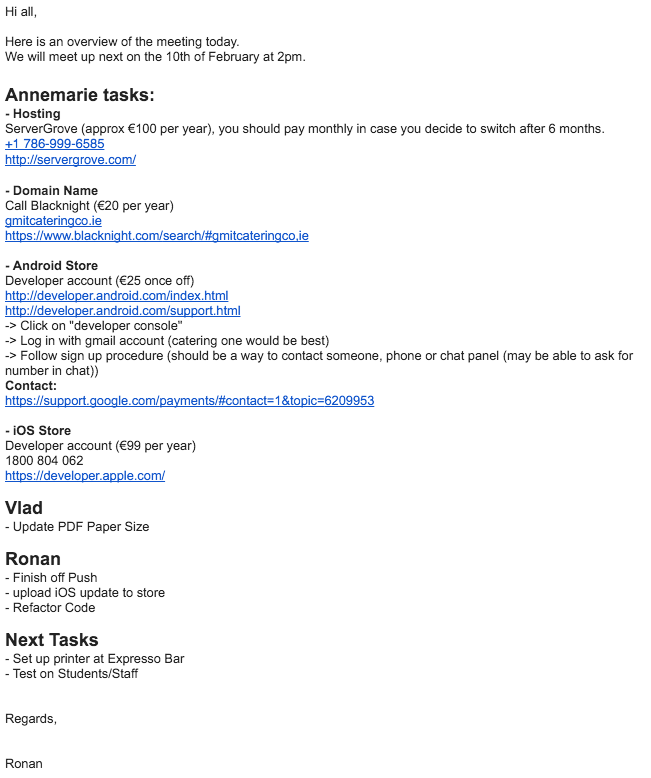
\includegraphics[width=1.0\linewidth]{img/2016_Meeting_1_Minutes}}
	\caption{2016 Meeting \#1 - Minutes}
	\label{fig:speciation}
\end{figure}
\begin{figure}[H] 
	\center{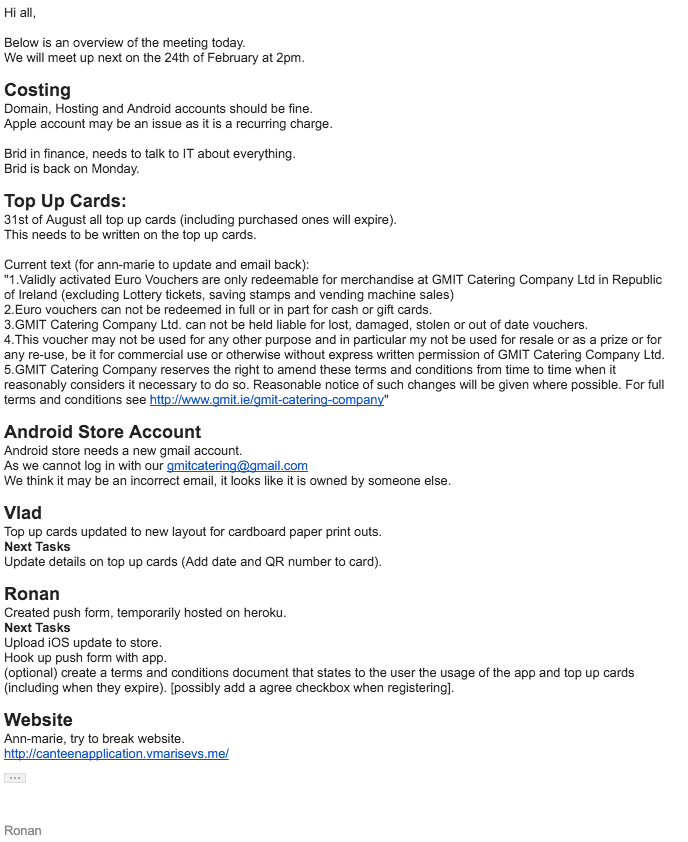
\includegraphics[width=1.0\linewidth]{img/2016_Meeting_2_Minutes}}
	\caption{2016 Meeting \#2 - Minutes}
	\label{fig:speciation}
\end{figure}

\subsection{Team Work}
We divided up all the work initially and along the way.
We used the GitHub issue tracker to flag bugs and highlight different improvements that could be made to the project.
We met up a few times a week to go through the project and make sure everything was syncing.
We learned much about working in teams from this project.

\section{Testing}
%What about validation and testing? Junit or some other framework.
Since there are so many different aspects to this project it was hard to bring in a testing framework.
I used created some test cases in Java with the Selenium WebDriver library in order to go through each tab of the web app and push server.
This helped us verify everything was working fine, we just needed to sit back and watch the test cases pass.
\\
For the mobile app I tried out Karma unit tests in conjunction with the Jasmine library.
We had an okay experience with this but we feel it is so cumbersome to set up that it may just be better to do user testing.
\\
We downloaded the mobile app on Android and iOS, and tested all the features out in various locations.
We did user testing by getting people from our year and the year below in software development and also some students who are not in the IT field to test all the features out and tell us the best and worst things they encountered within the application. 
This helped us improve the applications user experience, design and to kink our any bugs.
\\
We went through the web application with our client many times and updated it to make it easily usable for them.

\subsection{Test Server}
The test server contained all the routes necessary to mock the real server.
Here are the routes used:
	    \begin{table}[H]
	    	\centering
	    	\begin{tabular}{p{8cm}p{5cm}}
	    		\toprule \\
	    		\textbf{Route} & \textbf{Use} \\ \hline
	    		/ & Homepage \\  \hline
	    		/createuser/[data] & New User \\ \hline
	    		/verifyuser/[data] & Login \\ \hline
	    		/getfood & Get Menu \\ \hline
	    		/userhistory/[data] & Get User History \\ \hline
	    		/buyfood/[data] & Order Food \\ \hline
	    		/changeuserpw/[data] & Change Password \\ \hline
	    		/workingtime/[data] & Opening Times \\ \hline
	    		/topup/[data] & Topup Account\\ \hline
	    		/recoveruserpw/[data] & Reset Password \\ \hline
	    		\bottomrule
	    	\end{tabular}
	    	\caption{Routes table}
	    	\label{table:RoutesTable}
	    \end{table}
This is actually a good place to get a simple overview of how the real server works.
This is our interface.
\\
In order to switch between the test and real server we only need to change one line of code.
This file is located in:
\\
www/app/app.js
\begin{minted}[breaklines, mathescape, linenos, numbersep=5pt, frame=single, numbersep=5pt, xleftmargin=0pt]{css}
.constant('SERVER', {
  // test server
  // url: 'https://catering-test-server.herokuapp.com/',
  	
  // real server
  url: 'http://canteenapplication.vmarisevs.me/mobileapplication/',
});
\end{minted}
\section{Source Control}
%If team based, did you use GitHub during the development process.
We made sure to use source control throughout our project, utilizing branches and constant commits.
Between the mobile app and web app alone we have a total of \textbf{210} commits.

\subsection{GitHub}
We chose to use GitHub as our source control repository vendor as it is tried and trusted, we are used to it, we use it currently in college and it hosts some of the largest projects on the web. Also the issue tracker, wiki, web site builder and various other features are compelling.

\section{Choices}
%Selection criteria for algorithms, languages, platforms and technologies.
We already mentioned in the Context chapter about why we chose Ionic, Zend and Mean stack framework/architectures.
Here we will discuss why we chose PHP, SQL, JavaScript and JSON as our core technologies.
\subsection{PHP}
PHP is server side scripting language that is widely used and specially suited for web development it can be embedded into html page.

\begin{minted}{php}
<!DOCTYPE HTML>
<html>
   <head>
      <title>Example</title>
   </head>
   <body>
	
      <?php
         echo "Hi, I'm a PHP script!";
      ?>
	
   </body>
</html>
\end{minted}

It also has a wide range of protocols such as LDAP, IMAP, SNMP, NNTP, POP3, HTTP, COM and others, that can be used to talk to other services. PHP also has support for instantiation of Java objects and using them as native PHP objects.

\subsection{RDBMS (SQL)}
In order to chose between noSQL and RDBMS we thought about is there a reason why we should use SQL? Yes there is. In current project we are not just populating database with information, we also have to query the storage on the monotonic types, such as order date or all valid users. In this case we have large set of structured queries and Relational Database Management System can solve this problem. because one of their advantages is atomic transactions. This mean that if we have to do set of transactions and one of them fail then, all others will be canceled. NoSQL type databases are using eventual consistency that cannot at any time guarantee that at flow of transactions that comes together are all done at current point in time. If you will try to access data while transaction is in process you might receive corrupted data. 



\subsection{JavaScript}
JavaScript is the language that the Ionic and Angular core development team use for creating applications.
You can write any JavaScript from any framework in other languages like CoffeeScript or TypeScript.
\\

These follow stricter rules and allow JavaScript to be strongly typed.
This gives you auto-completion amongst other things.
It nearly a bit more like you're writing Java with these languages.
These languages are transpiled into JavaScript (as opposed to compiled).
\\
\textit{*The difference between transpiling and compiling is that transpiling compiles to the same abstraction level}.
\\

TypeScript and JavaScript are at the same abstraction level.
Transpiling is a form of compiling (a subset).
Transpilers are gaining popularity and often take the direction of up and coming standards.
If you learn Microsoft s TypeScript you are learning much of the new JavaScript standards to come.
\\
\textit{*TypeScript is being incorporated into Angular2.}
\\

If I were to do this project again in the future I would consider using TypeScript instead of JavaScript.

\subsection{JSON}
We chose to use JSON for passing messages between the mobile and web applications due to the fact that it is so lightweight and easy to create and parse.
Since the Ionic application is written with JavaScript it stores all it's data in JSON format by default.

PHP has a native function that parses object into JSON format string. In the example below we can see code snippet from Controller that prepares to return response back to user and in the content we are parsing array into JSON using \textit{json\_encode} function.
\begin{minted}{php}
<?php
public function indexAction{
  ...
  $response = $this->getResponse();
  $response->setStatusCode(200);        
  $response->setContent(json_encode($result_array));        
  return $response;
}
\end{minted}
\chapter{Technology Review} % 7-10 pages
% intro to tech review, bla bla bla
Here we will talk about all the technologies we used.

  \section{System Administration and Management Web Application}	% 4 pages
  After gathering all system requirements and we have done a research and based on them I decided to use PHP based framework because there is a lot of hosting companies that support this server scripting language and it has very cheap pricing.
  

    \subsection{php}
	PHP is in the market since 1995 and is one of the widely used server scripting language. It is quite powerful tool for making dynamic web pages and it is free. There are many popular websites that are written on \textbf{\textit{php}} such as Facebook, Wikipedia, Flickr, Mailchimp, Wordpress.com. PHP code can be embedded into html page. This type of structure allow to use it in various web template systems, content management systems or web frameworks. From beginning \textbf{\textit{php}} wasn't object oriented language, but in the later versions they redesigned it.

    \subsection{Zend Framework 2}
		Prototype was developed using \textbf{\textit{Zend Framework 2}}. This is an open source framework for developing Web applications and services. It was written on \textbf{\textit{php}} and it is loosely coupled architecture, which allow developer to code each component independently and designed with Model View Controller structure. \textbf{\textit{Zend Framework 2}} uses 100\% object-oriented code and utilises most of the new features of \textbf{\textit{PHP 5.3}}, namely namespaces, late static binding, lambda functions and closures.~\cite{ZendFramework-Website-About}
		
		%------------------------------------------
		\begin{wrapfigure}{r}{2.5cm}
			
\includegraphics[width=3cm]{img/zf2/zf2-logo.png}
		\end{wrapfigure} 
		%------------------------------------------
		Barry and Elhakeem~\cite{ZendFramework-Security-Model} argues that Zend Framework enables simple, rapid and agile web application development process, and it also offers AJAX support to convert XML data into JSON format and integrates the most widely used APIs and Web Services of third-party companies such as Google, Microsoft, Amazon, Flickr and Yahoo. ZF provides many options for validation such as Dojo tools it also allow to filter all inputs.
		
		%Zend Framework 2 is connected to a local MySQL relational database management system, to store the information about customers, orders and user accounts. The connection is established using ZF2 DB Adapter and Mysqli driver.
		
		%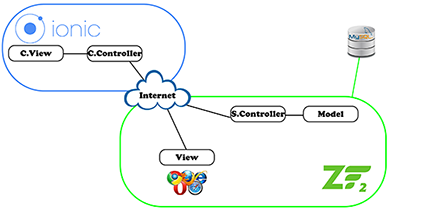
\includegraphics{img/zf2/ionic_zf2_mysql_diagram.png}
		
		Based on Hyun Jung La and Soo Dong Kim publication we can say that this project has a Balanced Model View Controller Architecture ~\cite{MVC_Architecture_for_Developing_Service-based_Mobile_Applications}. The \textbf{\textit{Zend Framework 2}} contains applications business logic or Model. And it is also responsible for validating user inputs or Server Side Controller and  Web application Views. While \textbf{\textit{Ionic}} is responsible for Client Side View and Controller (on the smartphone). In this case Mobile application uses \textbf{\textit{zf2}} Controllers to connect to \textbf{\textit{MySQL}} database.


			\subsubsection{QR code generator}
			QR codes are very popular type of two-dimensional barcode~\cite{QR_code_google}. This module was used for generating QR codes for vouchers. When voucher is printed users can scan this code and top up their balance. This module is overridden  for Zend Framework 2 and it uses Google Developers QR code generation API.~\cite{QR_code_generator}
			
			\subsubsection{DOM PDF module}
			In order to generate \textit{*.pdf} file we use DOM PDF module for Zend Framework 2. This is most common plugin that let me to solve problems with printing remote image. It is easy to use, because it parses HTML as DOM object and generates pdf file based on that.~\cite{DOM_PDF_module}

			\subsubsection{PDF make}
			In order to generate a large pdf file and move the heavy bit from hosting server, we are using JavaScript module that structures the information and generates the file.
			\cite{PDF_Make_module}
			
    \subsection{MySQL}
%------------------------------------------
\begin{wrapfigure}{r}{2.5cm}
	
\includegraphics[width=3cm]{img/zf2/mysql-logo.png}
\end{wrapfigure} 
%------------------------------------------
To store information we were using \textbf{\textit{MySQL}} database management system. It's reliability is proven through the years. \textbf{\textit{MySQL}} offers complete ACID (atomic, consistent, isolated, durable) transaction support, unlimited row-level locking, distributed capability, and multi-version transaction support where readers never block writers and vice-versa. Easy manageable platform that allow a DBA to manage, troubleshoot, and control the operation of many \textbf{\textit{MySQL}} servers from a single workstation. ~\cite{MySQL_Top10_Reasons}

    \subsection{Composer}
%------------------------------------------
\begin{wrapfigure}{r}{2.5cm}
	
\includegraphics[width=3cm]{img/zf2/composer-logo.png}
\end{wrapfigure} 
%------------------------------------------
For such large distributed projects like this more often used some sort of dependency managers, that allow to force the development cycle and reuse any of already written packages. One of the most popular dependency manager for \textbf{\textit{php}} is \textbf{\textit{composer}}.
After installing it we can start using it, simply by creating \textit{composer.json} file which describes the dependencies for your project and may contain other metadata as well.~\cite{Composer_doc} 

\textbf{\textit{composer.json}} example:

\begin{minted}{json}
{
    "require": {
        "php": ">=5.5",
        "zendframework/zendframework": "~2.5",
        "zendframework/zftool": "dev-master",
    }
}
\end{minted}

As you can see, require takes a key value pairs where key maps to package names and value is version of it. We also can configure the minimal supported release or nominal version. When \textit{composer.json} is completed, we can run command that will download chosen packages and configure them in our project. To do that run this command in console:
\begin{minted}{bash}
 $ php composer.phar update
\end{minted}

    \subsection{WAMP Server}
	WampServer is a Windows web development environment. It allows you to create web applications with Apache2, PHP and a MySQL database. Alongside, PhpMyAdmin allows you to manage easily your databases\cite{WAMPserver}. 
	
	%This software bundle allow you to setup any type of PHP services
	
    \subsection{Server Grove Hosting}
There is not so many hosting companies that supports Model View Controller structured \textbf{\textit{php}} websites, but the good old days when we were querying \textit{*.php} files are gone. This type of structure hides the extension and it will confuse the attacker on what sort of platform it was written.

One of most popular hosting companies in Ireland is Blacknight Solutions. For one of my portfolio websites I was using their services. At that time I was not bothered with developing my own website from the scratch and I have used \textit{Drupal} Content Management System. It is quite easy to install and setup CMS for lite blog type of website, but when it comes to connecting 2 different platforms it is no longer useful. When I developed my porfolio website on \textbf{\textit{zf2}} and tried to host it on their server I had a lot of issues with their policy. Customers don't have access to main \textit{php.ini} file which can change write properties that has to be on to use MVC structured websites. 

To solve this problems I have found \textit{Server Grove} hosting company that fully supports \textbf{\textit{Zend Framework 2}}, \textbf{\textit{Git Client}} and  \textbf{\textit{composer}}. It took me a while to move my domain name from BlackNight Solutions, but once I have it done all technical support on Server Grove is brilliant.


%\pagebreak
  \section{Mobile App} % 4 pages
The technology stack I chose to use for this project is quite extensive.  
Ionic is heavily based in the JavaScript community which is known for it's enormous amount of libraries and dependencies.
It is quite a steep learning curve to get to grips with the basics, and it takes quite a while to get comfortable in the workflow.
I came across a tweet that sums up this experience:
\begin{figure}[H] 
	\center{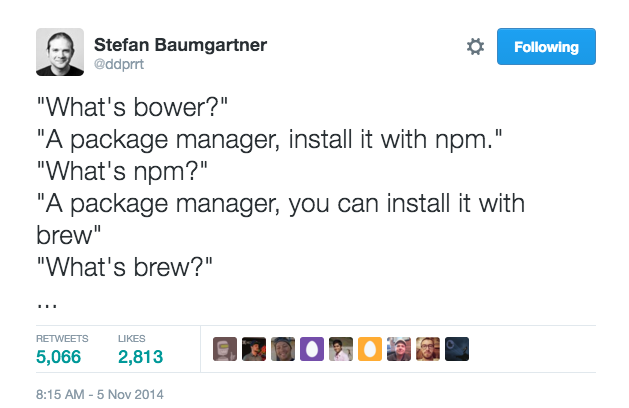
\includegraphics[width=0.8\linewidth]{img/mobile-app/js_dev_init}}
	\caption{JS Developer Learning Curve}
	\label{fig:speciation}
\end{figure}


I  done extensive research on different cross platform frameworks.
First I started with JQueryMobile and PhoneGap which had the capabilities but the community and tooling were quite scarce. 
\\ 

Xamarin was another option, It did not appeal to me as much, during my research I found many people had lots of issues with it and you still have to write some specific code for each platform.
\\ 

A lecturer of mine mentioned the Ionic framework to me and once I looked into it, it was the obvious choice.
Ionic has a huge community, extensive tooling for the majority of tasks needed and it is rapidly becoming the number one option for cross platform development.
\\

Once I had decided to take the Ionic route it meant that I was delving into the world of web development, as Ionic uses AngularJS, which is used with JavaScript, HTML, CSS and all the web development tools and work-flows.

\subsection{HTML/CSS}
\begin{wrapfigure}{r}{2.5cm}

\includegraphics[width=3cm]{img/mobile-app/logos/html-css.jpg}
\end{wrapfigure} 
I found that learning HTML \cite{html} and CSS \cite{css} was fine, I just needed to know enough to use Angular, which is very basic.
I had done some HTML and CSS before so I just needed to brush up on my skills.
I took the Web Development \cite{codeschool_webdev} course on Code School which helped me quickly get up to speed.
\\

HTML is great because it is a simple structure that is easy to understand.
It is just a subset of XML for websites.
\\

CSS makes is really easy to change various parts of the HTML form one place.
I used SASS (Sassy CSS), this lets you use CSS in a programmatic way (using variables).
\\

Here is a piece of SASS for the Ionic colours:
\begin{minted}[breaklines, mathescape, linenos, numbersep=5pt, frame=single, numbersep=5pt, xleftmargin=0pt]{css}
$light:                           #fff !default;
$stable:                          #f8f8f8 !default;
$positive:                        #5475aa !default; 
$calm:                            #11c1f3 !default;
$balanced:                        #7baa1e !default; 
$energized:                       #ffc900 !default;
$assertive:                       #840018 !default;
$royal:                           #886aea !default;
$dark:                            #444 !default;

// The path for our ionicons font files
$ionicons-font-path: "../lib/ionic/fonts" !default;

// Include all of Ionic
@import "www/lib/ionic/scss/ionic";

// custom styles
@import "scss/styles";
\end{minted}
You can also see that I am importing other style sheets.


\subsection{JavaScript}
\begin{wrapfigure}{r}{2.5cm}

\includegraphics[width=3cm]{img/mobile-app/logos/JS.png}
\end{wrapfigure} 
Once I had gotten myself into the basic mindset of HTML and CSS I decided to learn JavaScript.
I completed three JavaScript courses \cite{codeschool_js} on Code  School.
This gave me a great understanding of JavaScript \cite{javascript}.
\\
I found that JavaScript's event based nature took awhile to get the hang of but once understood it was very useful. 
Promises are a very important concept to understand as JS is asynchronous and tasks may not execute in order, especially blocking tasks.
This is useful as you don't need to code in concurrency, it is an inherent feature of the language.
\\
I wrote a literature review on using JavaScript for full stack development \cite{js_advantages_full_stack}, this touches on promises, the event based nature, and why JavaScript is so popular.

\subsection{AngularJS}
\begin{wrapfigure}{r}{2.5cm}
	
\includegraphics[width=3cm]{img/mobile-app/logos/angular.jpg}
	\centering
\end{wrapfigure}

I completed two AngularJS \cite{angular} courses on Code School. 
Then for each course I completed I done the 2/3 hour screen cast that accompanied it.
\\
The main problem I found with JavaScript is a lack of standards and structure. 
This is why I believe there are so many JS frameworks out there.
\begin{figure}[H] 
	\center{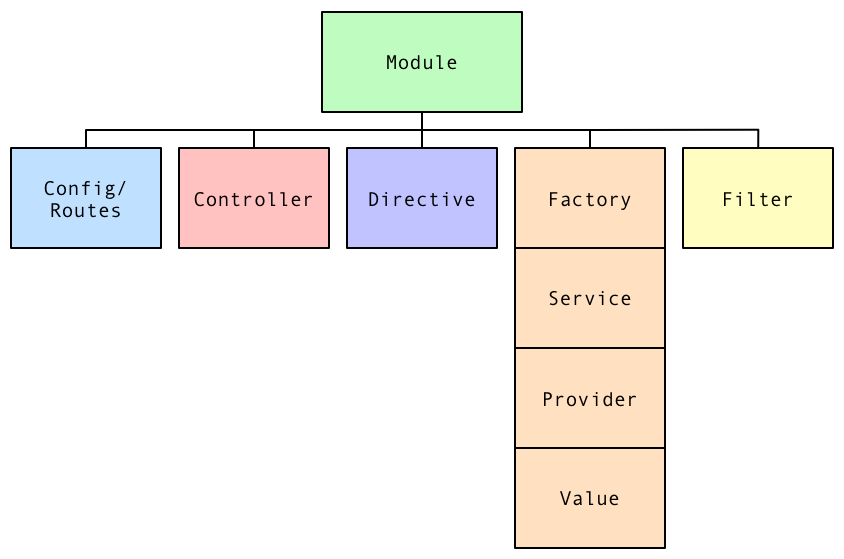
\includegraphics[width=0.75\linewidth]{img/mobile-app/angular_object_diagram.png}}
	\caption{Angular Object Diagram}
	\label{fig:speciation}
\end{figure}
A few times a year there a a new JS framework that all the web developers think is going to be the \textbf{one}.
AngularJs has risen and is now one of the top JS frameworks, partly I'm sure to do with the fact that Google is the project owner.
Competition includes Facebook's React \cite{react} and EmberJS \cite{ember}.
\\

I completed two Angular courses on Code School. 
Then for each course I completed I done the 2/3 hour screen cast that accompanied it.
\\

These helped me gain a deep understanding of controllers, services, routing and views.
Angular is based around the Model View Controller (MVC) model, where the design, data and logic are all separated.
\\
Angular is a Single Page Application (SPA). Only one page ever exists, the \textit{index.html}, then each \textit{view} is loaded into a section of this page.
Each \textit{view} has a \textit{controller} attached to it. 
The Modal contains the data which is loaded into a template that you code, this creates the view.

Two way binding is used so that as you enter information is can be seen straight away.
\begin{figure}[H] 
	\center{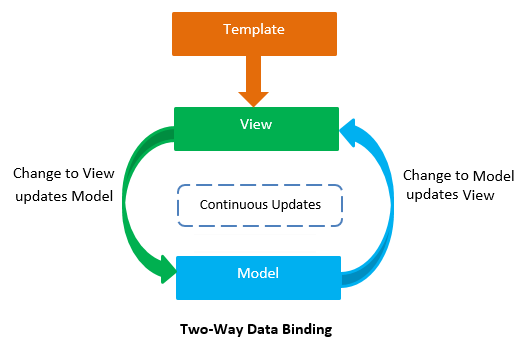
\includegraphics[width=0.75\linewidth]{img/mobile-app/two-waybinding.png}}
	\caption{Two Way Data Binding}
	\label{fig:speciation}
\end{figure}

%\pagebreak
\subsection{Ionic Framework}
% talk about JS, AngularJS, CSS, HTML and Ionic.
\begin{wrapfigure}{r}{2.5cm}
	
\includegraphics[width=3cm]{img/mobile-app/logos/ionic.png}
\end{wrapfigure} 
Once I understood AngularJS I completed some Ionic tutorials on \url{EggHead.io} and \url{Thinkster.io}.

The Ionic \cite{ionic} community is really great, the forum is very engaging, questions are answered very quickly and they post to their blog regularly.
The  founders Max Lynch, Adam Bradley and Ben Sperry talk about various updates every few months on YouTube, they call this \textit{The Ionic Show} \cite{ionic_show}.
\\

To Start an Ionic application you run these commands in bash:
\begin{minted}[%
breaklines,
mathescape,
linenos,
numbersep=5pt,
frame=single,
numbersep=5pt,
xleftmargin=0pt,
]{bash}
$ ionic start myApp tabs
$ cd myApp
$ ionic platform add ios
$ ionic build ios
$ ionic emulate ios
\end{minted}
Everything is done through command line.


\pagebreak
Here is a simple controller:
\begin{minted}[%
breaklines,
mathescape,
linenos,
numbersep=5pt,
frame=single,
numbersep=5pt,
xleftmargin=0pt,
]{js}
(function() {
    'use strict';

    angular
        .module('canteen.controllers')
        .controller('AboutCtrl', about);

    about
        .$inject = ['$scope', 'Orders'];

    function about($scope, Orders) {
        $scope.opening = Orders.opening;
        $scope.closing = Orders.closing;
        $scope.times = Orders.collTimes;
    }
})();
\end{minted}
One issue I came across is that there is no definitive way to lay out structures.
This is a common issue in JavaScript, since the standards are so loose (which benefits it in order ways).
\\

The above layout follows John Papas AngularJS style guide \cite{angular_style_guide}.
John Papa works with the Microsoft team who are implementing strong typing into Angular2 (through the use of MS TypeScript).
This gives me the impression that he has a good grasp on best design practices.
\\

As you can see in the above example, I have broken up the code into its constituent components, rather then the usual nested JavaScript hierarchy.
I think it is pleasing to the eye and easy to understand.

\subsection{Heroku}
\begin{wrapfigure}{r}{2.5cm}
	
\includegraphics[width=3cm]{img/mobile-app/logos/heroku.jpg}
\end{wrapfigure} 
We used Heroku \cite{heroku} to host the push and test servers.
Heroku is great for RAD, it is so simple to get a project live.
It treats the project that is hosted as a git repository.

In order to use Heroku you:
\begin{itemize}
	\item Install the Heroku Tool-belt
	\item Create a Procfile
	\item Initialize a Git repository
	\item Create a Heroku project via command line
	\item Commit and Push to the Heroku remote
\end{itemize}

\textbf{Here are the commands to create a new server and push to it} (once pushed it goes live instantly):
\begin{minted}[breaklines, mathescape, linenos, numbersep=5pt, frame=single, numbersep=5pt, xleftmargin=0pt]{bash}
> heroku login
> git init
> heroku create
> git add .
> git commit -a
> git push heroku master
> heroku open
\end{minted}

\textbf{Here is the Procfile} (this is the Heroku config file for the project, here we give the server the command to start our project):
\begin{minted}[breaklines, mathescape, linenos, numbersep=5pt, frame=single, numbersep=5pt, xleftmargin=0pt]{yaml}
web: node server.js
\end{minted}

\section{Stores}
We decided to release the application on the iOS and Android stores.
\\

\href{https://itunes.apple.com/ie/app/gmit-catering/id1054850061?mt=8}{iOS App Store Link}.

\href{https://play.google.com/store/apps/details?id=ie.gmit.catering}{Android App Store Link.}

\subsection{iOS Store}
\begin{wrapfigure}{r}{2.5cm}
	
\includegraphics[width=3cm]{img/mobile-app/logos/ios.png}
\end{wrapfigure} 
Apples iOS store \cite{ios} is tricky to get used to, first you must submit an application for a developer account which costs €99 per year. They require much information. Once complete you have to create a developer certificate, provisioning profile, push notification certificate, download them, and sign them locally. You have to get these certificates for both production and development purposes, as Apple see these as completely separate applications.
\\

Once complete you install XCode (for developing iOS apps), compile the application, login to your profile in XCode, go through the local setup, then archive the application in XCode and submit this to the store (through XCode). After a few hours you get an email saying that the Archive is okay. You then go to the ITunesConnect website, login, and start the store application process, this takes numerous steps.
\\
Once complete you can add the previous archived file and submit for approval to the store, this takes 1 to 2 weeks to complete, often resulting in a change wish the revision team want to see updated. You must provide the revision team with a mock account to test the application.
\\
I got used to this process after my third or fourth update.
\\
This process results in only top quality applications making it into the iOS stores.
The iOS store makes more money then the Android store by a long shot.

\subsection{Android Store}
\begin{wrapfigure}{r}{2.5cm}
	
\includegraphics[width=3cm]{img/mobile-app/logos/android.png}
\end{wrapfigure} 
Submitting an app to the Android \cite{android} (Google Play) store is a joy.
First you go to the Google Play website, login with your Google account, give some extra details, pay €25 (per year) and you are instantly in.
You then click on "create new app", fill out some details and it asks for the app binary file.
\\
In order to generate the Android binary file you must create a local android keystore (for signing ) compile the app with the Ionic tool, sign it, zipalign it and then submit it to the Google play store.
You submit it by simply dragging it into the Google Play web site window. Within two hours the application will be live.

I looked into why it's so quick, and apparently they test your application after it is submitted, this leads to happy developers.

Here is the bash script I create to automate the Android build process:
\begin{minted}[breaklines, mathescape, linenos, numbersep=5pt, frame=single, numbersep=5pt, xleftmargin=0pt]{bash}
#! /usr/bin/env sh

ionic build android --release
rm gmitcat.apk
cp platforms/android/build/outputs/apk/android-release-unsigned.apk .

jarsigner -verbose -sigalg SHA1withRSA -digestalg SHA1 -keystore ./ronanc.keystore android-release-unsigned.apk ronanc

zipalign -v 4 android-release-unsigned.apk gmitcat.apk

cp gmitcat.apk ~/Dropbox/releases/
\end{minted}
\textit{*I couldn't do this for iOS as you need to use XCode.}

\subsection{Windows Phone Store}
\begin{wrapfigure}{r}{2.5cm}
	
\includegraphics[width=3cm]{img/mobile-app/logos/windows.png}
\end{wrapfigure} 
The Windows Phone store \cite{windows_phone} is actually not that bad, I have already submitted 36 applications (mostly micro applications) to this store.
It's free to sign up and the set-up process is very simple, lots of check-boxes and drop-down menus.
\\
The reason we didn't create a Windows Phone version is that firstly it is not supported by Ionic. Cordova (which Ionic is based on) does support it, but to get it working takes a lot of work, and we felt that the market for Windows Phone users is so small that it was not worth our time.
\\
Ionic2 will be supporting Windows Universal Platform applications, so in the future this application could be migrated to the Windows Platform quite easily.

\section{JS Tools}
\subsection{Yeoman}
\begin{wrapfigure}{r}{2.5cm}

\includegraphics[width=3cm]{img/mobile-app/logos/yeoman.png}
\end{wrapfigure}
\cite{yeoman}
We used Yeoman to scaffold out the push web application.  
There were some dependency issues, which are not uncommon with NPM.
Once these were solved we used Yeoman's Angular Generator \cite{angular_generator} to scaffold out a skeleton.
\\
Since there are so many frameworks, plug-ins and libraries in the web development community, a tool like this is needed to bring some structure to the chaos of this heterogeneity. It is analogous to a command line wizard.
 \\
 Here is the output when using the Angular Generator:
\begin{minted}[breaklines, mathescape, linenos, numbersep=5pt, frame=single, numbersep=5pt, xleftmargin=0pt]{bash}
Ronan:~/development/misc$ yo angular

_-----_
|       |    .------------------------------------------.
|--(o)--|    | Update available: 1.7.0 (current: 1.6.0) |
`---------´   |     Run npm install -g yo to update.     |
( _´U`_ )    '------------------------------------------'
/___A___\
|  ~  |
__'.___.'__
´   `  |° ´ Y `


_-----_
|       |    .--------------------------.
|--(o)--|    |    Welcome to Yeoman,    |
`---------´   |   ladies and gentlemen!  |
( _´U`_ )    '--------------------------'
/___A___\
|  ~  |
__'.___.'__
´   `  |° ´ Y `

Out of the box I include Bootstrap and some AngularJS recommended modules.

? Would you like to use Gulp (experimental) instead of Grunt? No
? Would you like to use Sass (with Compass)? No
? Would you like to include Bootstrap? Yes
? Which modules would you like to include? angular-animate.js, angular-cookies.js, angular-resource.js, angular-route.js, angular-sanitize.js, angular-touch.js
create app/styles/main.css
create app/index.html
create bower.json
create .bowerrc
create package.json
create Gruntfile.js
create README.md
invoke   angular:common:/usr/local/lib/node_modules/generator-angular/app/index.js
create     .editorconfig
...

I'm all done. Running bower install & npm install for you to install the required dependencies. If this fails, try running the command yourself.
 \end{minted}
As you can see straight away, we are not on the current version.
The \textit{create} commands are the files that are created, you can kind of get an idea of the structure from that.
\\

Once \textit{bower install \& npm install} we ran we were met with this:
\begin{minted}{bash}
misc@ /Users/Ronan/development/misc
UNMET PEER DEPENDENCY grunt@>=0.4.x
|-> grunt-karma@0.12.2
    |->lodash@3.10.1
|-> UNMET PEER DEPENDENCY jasmine-core@*
|-> UNMET PEER DEPENDENCY karma@^0.13.0 || >= 0.14.0-rc.0
|->  karma-jasmine@0.3.8
|->  karma-phantomjs-launcher@1.0.0
    |->  lodash@4.11.1
|-> UNMET PEER DEPENDENCY phantomjs-prebuilt@>=1.9
 \end{minted}
These kinds of errors are common and usually the answer is found in the comment thread of the projects GitHub Issue Tracker.

This can take up to five minutes to complete installing.

Once installed we have a project that has grunt, jasmine, karma, bower and an angular application ready to go!
This would usually take much longer to set-up.
We went out and learned each of these technologies individually before using this generator, otherwise you don't understand what's happening.

\subsubsection{Grunt}
\begin{wrapfigure}{r}{2.5cm}

\includegraphics[width=3cm]{img/mobile-app/logos/grunt.png}
\end{wrapfigure} 
Grunt \cite{grunt} is a task runner like \textit{Ant} or \textit{Gulp}.
It runs various tasks for you.
It is needed when you have multiple steps in your project.
Below are a few parts to the \textit{GruntFile.js} from the push web app.
\\

\textbf{Registering some tasks:}
\begin{minted}{bash}
  grunt.registerTask('test', [
  'clean:server',
  'wiredep',
  'concurrent:test',
  'postcss',
  ]);
  
  grunt.registerTask('default', [
  'newer:jshint',
  'newer:jscs',
  'test',
  'build'
  ]);
\end{minted}
  
\textbf{Here is one of those tasks:}
  \begin{minted}{bash}
// Empties folders to start fresh
clean: {
    dist: {
        files: [{
            dot: true,
                src: [
                    '.tmp',
                    '<%= yeoman.dist %>/{,*/}*',
                    '!<%= yeoman.dist %>/.git{,*/}*']
                }]
        },
    server: '.tmp'
},
  \end{minted}
  
 \textbf{To run grunt you type one of the below commands:}
  \begin{minted}{bash}
> grunt
> grunt build
> grunt test
  \end{minted}
  Running \textit{grunt} is the same as tunning \textit{grunt default}.
 
 \subsection{Gulp}
 \begin{wrapfigure}{r}{2.5cm}
 	
\includegraphics[width=3cm]{img/mobile-app/logos/gulp.png}
 \end{wrapfigure} 
As said before, Gulp \cite{gulp} is like Grunt.
The main difference is that Gulp is programmatic rather then defined.
\\
We are using it for SASS \cite{sass} here.
SASS is framework that allows one to write CSS in a programmatic way.
\\
\textbf{Example from the Ionic App (\textit{gulpfile.js}):}
\begin{minted}[breaklines]{js}
// imports

var paths = {
sass: ['./scss/**/*.scss']
};

gulp.task('default', ['sass']);

gulp.task('sass', function(done) {
gulp.src('./scss/ionic.app.scss')
.pipe(sass())
.pipe(gulp.dest('./www/css/'))
.pipe(minifyCss({
keepSpecialComments: 0
}))
.pipe(rename({ extname: '.min.css' }))
.pipe(gulp.dest('./www/css/'))
.on('end', done);
});

gulp.task('watch', function() {
gulp.watch(paths.sass, ['sass']);
});

gulp.task('install', ['git-check'], function() {
return bower.commands.install()
.on('log', function(data) {
gutil.log('bower', gutil.colors.cyan(data.id), data.message);
});
});

// error stuff
done();
});
\end{minted}

\subsection{Jasmine}
\begin{wrapfigure}{r}{2.5cm}

\includegraphics[width=3cm]{img/mobile-app/logos/jasmine.png}
\end{wrapfigure} 
\cite{jasmine}
Jasmine is just a bunch of functions that test your code.
You give it an input or action and state what the result should be.
Much like \textit{JUnit}, Jasmine is unit testing.
\\

It is a behaviour driven development framework for testing JavaScript code, and is doesn't rely on any other JavaScript frameworks.
\\ 

\textbf{Here is a sample test for the home controller on the push web app:}
  \begin{minted}{js}
'use strict';

describe('Controller: HomeCtrl', function () {

// load the controller's module
beforeEach(module('gmitcat'));

var HomeCtrl,
scope;

// Initialize the controller and a mock scope
beforeEach(inject(function ($controller, $rootScope) {
    scope = $rootScope.$new();
    HomeCtrl = $controller('HomeCtrl', {
    $scope: scope
    // place here mocked dependencies
});
}));

it('should attach a list of awesomeThings to the scope', function () {
    expect(HomeCtrl.awesomeThings.length).toBe(3);
});
});
\end{minted}

We didn't incorporate many of these tests, as we did extensive user testing and only rely looked into this near the end of the project, but in future projects I would implement this from the get go.

\subsection{Karma}
\begin{wrapfigure}{r}{2.5cm}

\includegraphics[width=3cm]{img/mobile-app/logos/karma.png}
\end{wrapfigure} 
\cite{karma}
Karma is test-framework agnostic, what is does is spawn a web server that executes test code against source code for each of the browsers connected. You can plug any compatible testing-framework into this. Examples are: Jasmine, Mocha, and QUnit.

Once Karma is installed (via NPM) you just need to setup the config file and choose a testing framework.
\\

\textbf{Here is part of our Karma Config file for the Push Web App}:
\begin{minted}
[breaklines, mathescape,, numbersep=5pt, numbersep=5pt, xleftmargin=0pt]
{bash}
module.exports = function(config) {
config.set({

// list of files / patterns to load in the browser
files: [
// bower:js
'app/scripts/**/*.js', 'test/mock/**/*.js', 'test/spec/**/*.js'
],
port: 8080,

// - Chrome, ChromeCanary, Firefox, Opera, Safari (only Mac), PhantomJS, IE (only Windows)
browsers: [
'PhantomJS'
],

plugins: [
'karma-phantomjs-launcher', 'karma-jasmine'
],
singleRun: false,
colors: true,

// level of logging
// possible values: LOG_DISABLE || LOG_ERROR || LOG_WARN || LOG_INFO || LOG_DEBUG
logLevel: config.LOG_INFO,
});
};
\end{minted}

\subsection{Bower}
\begin{wrapfigure}{r}{2.5cm}

\includegraphics[width=3cm]{img/mobile-app/logos/bower.png}
\end{wrapfigure} 
Bower \cite{bower} is a package manager like \textit{Maven} or \textit{NPM}.
It is often used in conjunction with NPM.
The main difference is the way it loads packages into an application.
\\
Bower loads items via dependency injection in the \textit{app.js file}.
We can see below the angular-md5 package being loaded in along with some default.
\begin{minted}[breaklines]{js}
angular
.module('canteen', ['ionic', 'ionic.service.core', 'canteen.controllers', 'canteen.services', 'ngCordova', 'ngMessages', 'angular-md5']);
\end{minted}

Below is the list of dependencies for the project, these get install when the command: \textit{bower.json} is run.
\\

\textbf{\textit{bower.json file} from the Ionic app:}
\begin{minted}{js}
{
    "name": "GmitCatering",
    "private": "true",
    "devDependencies": {
        "ionic": "driftyco/ionic-bower#1.1.0",
        "platform.js": "platform#~1.3.0",
        "ionic-platform-web-client": "~0.2.1"
    },
    "dependencies": {
        "angular-md5": "~0.1.10"
    }
}
\end{minted}

\subsection{NPM}
\begin{wrapfigure}{r}{2.5cm}

\includegraphics[width=3cm]{img/mobile-app/logos/npm.png}
\end{wrapfigure} 
NPM \cite{npm} is the main package manager for nearly all JavaScript projects, including Ionic.
It is similar to Bower.

Below is the list of dependencies for the Ionic application:
\begin{minted}{js}
{
"name": "gmitcatering",
"version": "1.0.0",
"description": "GmitCatering: Purchase food with ease",
"dependencies": {
"cordova": "^5.3.3",
"gulp": "^3.5.6",
"gulp-concat": "^2.2.0",
"gulp-minify-css": "^0.3.0",
"gulp-rename": "^1.2.0",
"gulp-sass": "^2.0.4"
},
"devDependencies": {
"bower": "^1.3.3",
"gulp-util": "^2.2.14",
"shelljs": "^0.3.0"
},
"cordovaPlugins": [
"cordova-plugin-whitelist@1.0.0",
"phonegap-plugin-push"
],
"cordovaPlatforms": [
"android",
"ios"
]
}
\end{minted}

Here we are loading some NPM modules into the gulp file for use:
\begin{minted}{js}
var gulp = require('gulp');
var gutil = require('gulp-util');
var bower = require('bower');
var concat = require('gulp-concat');
var sass = require('gulp-sass');
var minifyCss = require('gulp-minify-css');
var rename = require('gulp-rename');
var sh = require('shelljs');
\end{minted}

\subsection{BASH}
\begin{wrapfigure}{r}{2.5cm}

\includegraphics[width=3cm]{img/mobile-app/logos/bash.jpg}
\end{wrapfigure} 
As you can see throughout the document so far, we have used the terminal for many tasks, and even created some scripts.
BASH \cite{bash} is invaluable to the development work-flow, being able to group various commands into a file and just run the file is a great way to encapsulate processes. 

\section{Web App Alternatives}
% alternatives? JQueryPhone, PhoneGap, Cordova, Xamarin
\subsection{Cordova}
\begin{wrapfigure}{r}{2.5cm}

\includegraphics[width=3cm]{img/mobile-app/logos/cordova.jpg}
\end{wrapfigure} 
Cordova \cite{cordova} is an amazing project which gives us the ability to develop a mobile application from a single web view.
Cordova allows us to access hardware on the device that would otherwise be very tricky.
\\

They support:
\begin{itemize}
\item iOS
\item Android
\item Windows Phone
\item BlackBerry
\item UbuntuPhone
\item FirefoxPhone
\item LGwebOS
\item FireOS
\end{itemize}

Ionic is based on Cordova.

\subsection{PhoneGap}
\begin{wrapfigure}{r}{2.5cm}

\includegraphics[width=3cm]{img/mobile-app/logos/PhoneGap.png}
\end{wrapfigure} 
Adobe own PhoneGap \cite{phonegap}, when they purchased the Cordova project, some aspects had to be kept open source.
Adobe has created some great services and proprietary APIs for Cordova.

\subsection{JQueryMobile}
\begin{wrapfigure}{r}{2.5cm}

\includegraphics[width=3cm]{img/mobile-app/logos/jquery-mobile.png}
\end{wrapfigure} 
JQuery \cite{jquery_mobile} Mobile helps you create JavaScript interfaces for mobile apps and mobile web apps.
It can be used with PhoneGap or many other frameworks.
Check \href{http://jquerymobile.com/resources/}{this website} out to view all available frameworks.
\\
I probably would of went for this library mixed with Cordova if Ionic was not available.
Although it is way behind in many aspects.

\subsection{Xamarin}
\begin{wrapfigure}{r}{2.5cm}

\includegraphics[width=3cm]{img/mobile-app/logos/xamarin.png}
\end{wrapfigure} 
\cite{xamarin}
Xamarin is a great choice for developers who want to create cross platform applications in C\#, or for those who really don't like the JavaScript world.
You code your Windows Universal Platform application up in C\# and Xamarin will port your \textbf{Core Logic} to Android and iOS.
You still have to write the View layer and Native API layers yourself though.
\\

We found after talking to the community on the forums that it was quite buggy and there wasn't much support in some areas.
For instance the ported code is usually very different then if you were to create it yourself in Android or iOS so it's very hard to ask for help as all of your code will be completely custom.

  \section{Push Web Application}
The Push Web App uses AngularJS, NodeJS, ExpressJS, Cloudant and Heroku.
We chose to use these technologies as we needed to quickly create a server to facilitate push notifications.
We did not realise that we would need to store a list of device tokens, and it was too late to update the SQL Schema.

\subsection{CouchDB/Cloudant}
\begin{wrapfigure}{r}{2.5cm}

\includegraphics[width=3cm]{img/mobile-app/logos/cloudant.jpg}
\end{wrapfigure} 
IBM's cloudant \cite{cloudant} NoSQL database solution usese CouchDB \cite{couchdb} as the database of choice.
It has a fantastic user interface and is a joy to use.
IBM also guarantee high levels of performance and very low downtime (SLA).
\\

The other alternative I thought of using was Google's Firebase.
I think these are both very good NoSLQL DB as a service solutions.
Another one that has been around for awhile is Mlab (MongoDB as a service).

\subsection{NodeJS}
\begin{wrapfigure}{r}{2.5cm}

\includegraphics[width=3cm]{img/mobile-app/logos/nodejs.png}
\end{wrapfigure} 
NodeJS \cite{nodejs} which I talk about in detail in my literature review \cite{js_advantages_full_stack} in detail, has taken the web by storm the past couple of years. It has allowed developers to bring JavaScript from the client side to the server side using Google's JavaScript interpreter (V8 Engine), this V8 Engine heavily optimizes the JS code and uses JIT compilation to give near native performance, this coupled with the event based nature (which removes the need for threads) makes it a strong choice for server side development.

\subsection{ExpressJS}
\begin{wrapfigure}{r}{2.5cm}

\includegraphics[width=3cm]{img/mobile-app/logos/express.png}
\end{wrapfigure} 
ExpressJS \cite{expressjs} is a web development framework based on the NodeJS environment, it abstracts many common tasks into functions, like setting up a web server or HTTP RESTful routes.
\\
Here is an example of a simple ExpressJS HTTP Server with RESTful home route:
\begin{minted}{js}
var express = require('express');
var app = express();

app.set('port', (process.env.PORT || 5000));

// home page
app.get('/', function(req, res){
    var result = {"message": "Welcome to the gmit catering api"};
    res.contentType('application/json');
    res.send(JSON.stringify(result));
});

app.listen(app.get('port'), function() {
    console.log('Node app is running on port', app.get('port'));
});
\end{minted}

  %\pagebreak
  \section{GitHub}
  \begin{wrapfigure}{r}{2.5cm}
  	
\includegraphics[width=3cm]{img/zf2/github-logo.png}
  \end{wrapfigure} 
  We used GitHub \cite{github} throughout our project in order to utilize source control and keeping track of versions.
  We found that it was very useful in that we could have separate repositories for the different parts of the project.
  When we did work on the same repository we each had our own branch to which we would merge intermittently into the \textit{master} branch.
  We also used the \textit{issue tracker} to raise any issues/bugs we noticed on each others projects, or to mention an enhancement that could be incorporated.
  
  \begin{figure}[H] 
  	\center{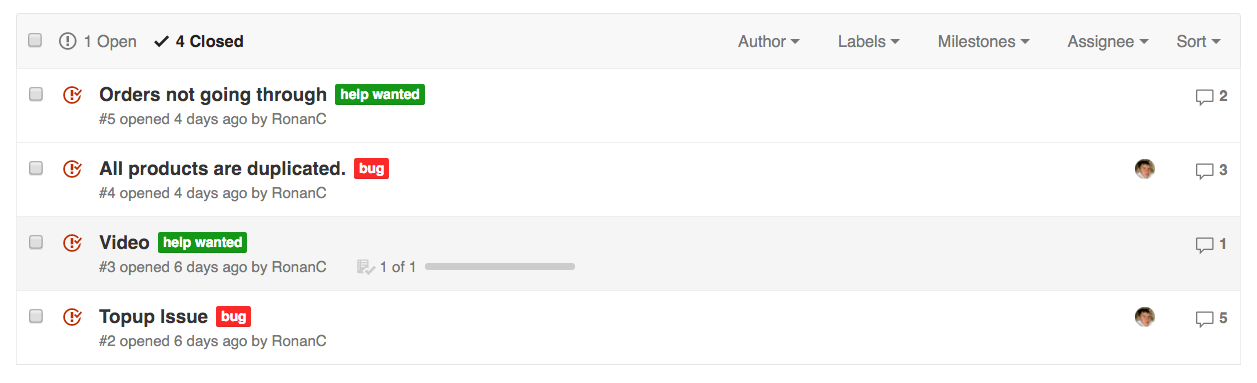
\includegraphics[width=1.0\linewidth]{img/issue_tracker}}
  	\caption{Issue Tracker}
  \end{figure}
  
  
  We also created an organisation, which acts as an entity.
  We forked all our repositories there and used it as a central hub for the overall project \cite{github_org}.
  \begin{figure}[H] 
  	\center{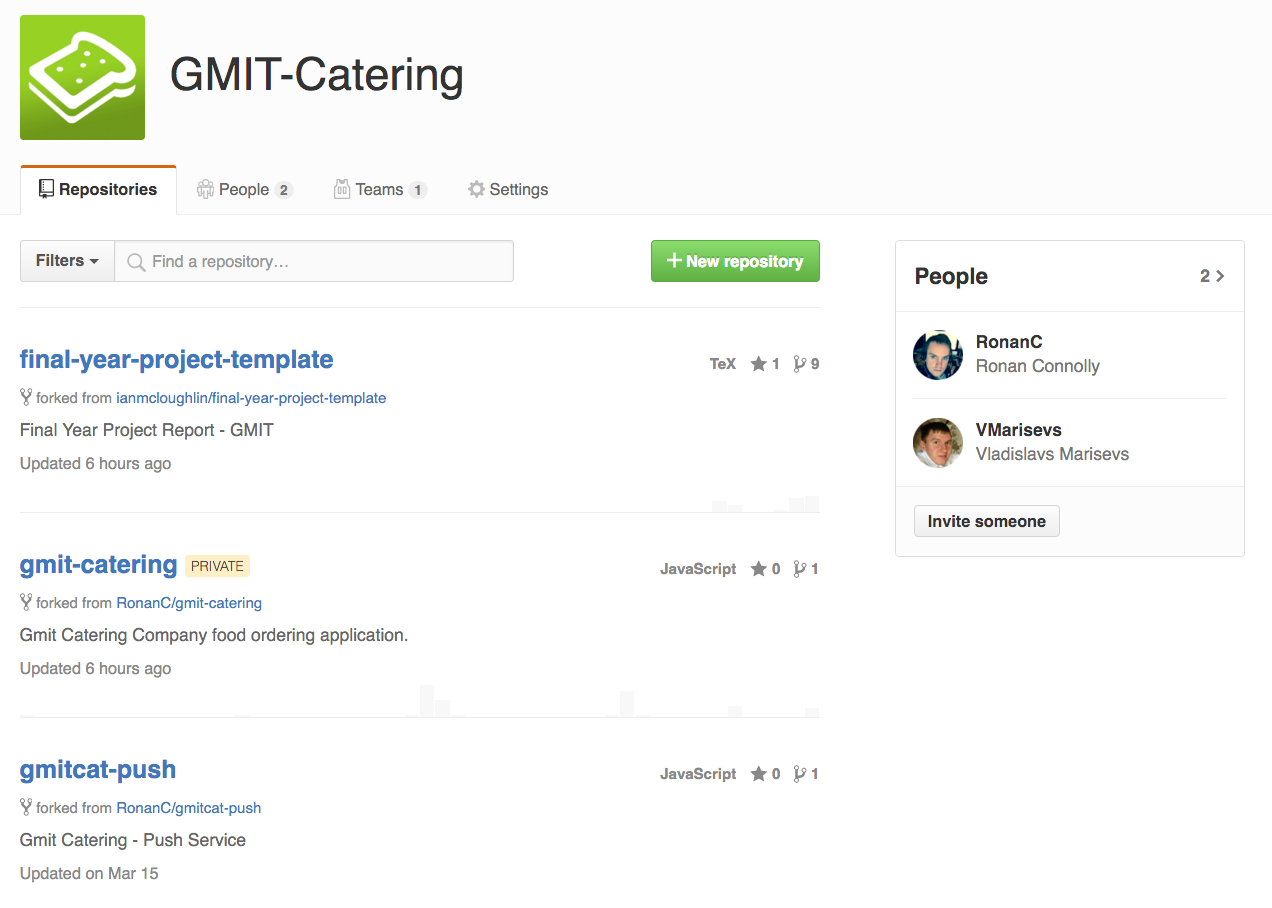
\includegraphics[width=1.0\linewidth]{img/github_org}}
  	\caption{GMIT Catering GitHub Org}
  	\label{fig:speciation}
  \end{figure}
  
  %\pagebreak
  \section{JSON REST interface architecture}	% 1 pages
  \begin{wrapfigure}{r}{2.5cm}
  	
\includegraphics[width=3cm]{img/mobile-app/logos/express.png}
  \end{wrapfigure} 
We chose to use a RESTful architecture   ~\cite{JSON_REST_interface} with JSON   \cite{json} because it is very simple and easy to understand and use.
It's reliable and has been battle tested with time.
\\
Both setting up and querying a RESTful system is trivial.
  
  \subsection{HTTP Requests}
  \begin{wrapfigure}{r}{2.5cm}
  	
\includegraphics[width=3cm]{img/mobile-app/logos/express.png}
  \end{wrapfigure} 
  \cite{http_methods}
  In order to query our RESTful system we used HTTP requests.
  These are very intuitive, they were designed to be common sense and simple to understand.
  \\
  Here is a list of HTTP Request Type:
	    \begin{table}[H]
	    	\centering
	    	\begin{tabular}{x{2cm}p{6cm}p{6cm}}
	    		\toprule \\
	    		\textbf{Name} & \textbf{Function} & \textbf{Example} \\ \hline
	    		Get & Gets the data at that URL & /users/Ronan OR /users/ \\ \hline
	    		Put & Updates the data at that URL & /users/Ronan \\ \hline
	    		Post & Saves a new user to a URL & /users/ \\ \hline
	    		Delete & Deletes the data at that URL & /users/Ronan \\ \hline    			    	    		
	    		\bottomrule
	    	\end{tabular}
	    	\caption{HTTP Requests}
	    	\label{table:HttpRequests}
	    \end{table}
    
  % talk about the HTTP get/post requests used via the interface from the phone and server
  \subsection{Custom API}
We created a Custom HTTP RESTful API on our web application.
It contains various routes which are discussed in the web app section of the system design and illustrated via angular HTTP code snippets in the mobile app section of the system design below.
\\

We found this to be very quick and easy to set up and would recommend it to others and we ourself would use it in the future without a doubt.
\\

The web server has a custom API that the mobile app uses
We will go into it some more below in the System Design section. 

\chapter{System Design}	% n-m pages
  \section{Database}
    \subsection{Purpose}

This section describes how the database that will support the system with details of the logical and physical definitions. It also provides the functional and non-functional usage of the tables, considerations and requirements.

The database design for the system is composed of definitions for db objects derived by mapping entities to tables, attributes to columns, unique identifiers to unique keys and relationships to foreign keys. 

Further in this document you will read the integration aspects of the Database with the Web Application and to understand them I want to explain some word definitions that will be used.
\\
\begin{itemize}
\item Customer is a physical person who uses smartphone application.

\item User is a physical person who operates with management website.

\item Food is entire product of this business.

\item Voucher is a printed card with unique code that allow customers to top up their account balance.
\end{itemize}
    \subsection{Procedures and Functions}
One of good reasons to use stored procedures is the added layer of security that can be placed on the database from the calling application. The risk of a attacker using the account to run a stored procedure that has been written by you is far safer than having the user account have full insert, update and delete authority on the tables directly. Another advantage to use stored procedures is the data functionality that is separated from the application making it easier to manage, document and maintain. They also improves the performance for example to make a payment I am doing just one call and DBMS can process it, which is more efficient than do complete processing on the php side.
\\

\begin{itemize}
	

\item \textbf{Verify Customer}
\\
This procedure takes two parameters login name and password, then parses it and returns the result. This procedure is used to connect Ionic application with DBMS and verify customer's credentials. If the password and login matches database returns complete details about current customer. This information can be displayed in the mobile application.

\item \textbf{Block Customer} 
\\
If system administrator sees that some user tried to enter invalid voucher id too many times, he can block this person. To keep a track of all invalid customer inputs I decided to add a basic counter, so that administrator can keep an eye on the malicious users that tries to insert voucher code permutations.

\item \textbf{Change customer's password}
\\
One of the common procedures when user is allowed to change their password if they are authorized.

\item \textbf{Insert customer}
\\
This procedure let people register their account as customer of the ordering system. To do that they have to insert their details, once that is done they can start using mobile application.

\item \textbf{Recover customer's password}
\\
In order to recover the password, user have to insert their email address and login. It will trigger the scenario of generating new temporary password for this user and will send it out to their email address. The procedure of sending emails from web application uses SMTP protocol, by default it is linked with gmail account. The settings are stored statically in configuration file \textit{*/config/autoload/email.local.php}. If login and email exists in the database it will save new password.


\item \textbf{Food insert}
\\
This procedure takes all food information, generates new identification number and returns it.


\item \textbf{Food update}
\\
In order to update the food, we are not overriding the record, but creating a new one with unique id and setting the original \textit{'active'} column to \textit{false}. This technique let us to keep track of all changes and prevent updates on the old orders.


\item \textbf{Delete Food}
\\
If user requires to remove the food, he is using this procedure. It just sets \textit{'active'} column to false and it will remove current food from list. But in case there was any orders with this food it will save a link and old details.


\item \textbf{Create order}
\\
This procedure will create an order in case it receives all valid information and returns new generated id or null which mean something is invalid.

\item \textbf{Food Order  Insert}
\\
When order is created and id returned, it starts filling it with products. 

\item \textbf{Order make payment}
\\
This procedure compares the balance on the account and if it is sufficient to make a payment it will deducts the money from user and mark the order as paid. These operations are separate to prevent incompleteness of the transaction. 

\item \textbf{Order price}
\\
This procedure calculates sum of order items and returns it.

\item \textbf{Order cancel payment}
\\
To cancel order payment we have to calculate sum of item prices and return them to customers balance.

\item \textbf{Create voucher}
\\
This function generates new voucher and places it in database.

\item \textbf{Topup customer account}
\\
Current transaction marks the voucher with customers account identification and adds money to their balance. After that this id is no longer valid for next transaction.


\end{itemize}
 
    \subsection{Tables}
    
    \subsubsection{Order System}
	    
Ionic application users table:	    
	    % Customers
	    \begin{table}[H]
	    	\centering
	    	\begin{tabular}{x{2cm}p{3cm}}
	    		\toprule \\
	    		\textbf{Column} & \textbf{Type} \\ \hline
	    		id & binary(16) \\ \hline
	    		gnumber & int(11) \\ \hline
	    		email & varchar(40) \\ \hline
	    		password & char(41) \\ \hline
	    		cash & decimal(13,2) \\ \hline
	    		active & tinyint(1) \\ \hline
	    		created & datetime \\ \hline
	    		updated & timestamp \\ \hline
	    		name & varchar(40) \\ \hline
	    		surname & varchar(40) \\ \hline
	    		address & text \\ \hline
	    		mobile & varchar(10) \\ \hline
	    		cheat & int(10) \\
	    		\bottomrule
	    	\end{tabular}
	    	\caption{Customers table}
	    	\label{table:CustomersTable}
	    \end{table}
    
    
Vouchers table:	    
	% Vouchers
	\begin{table}[H]
		\centering
		\begin{tabular}{x{2cm}p{3cm}}
			\toprule \\
			\textbf{Column} & \textbf{Type} \\ \hline
			id & varchar(16) \\ \hline
			amount & decimal(13,2) \\ \hline
			used & tinyint(1) \\ \hline
			customer & binary(16) \\ \hline
			activated & datetime \\ \hline
			created & datetime \\ \hline
			modified & timestamp \\
			\bottomrule
		\end{tabular}
		\caption{Vouchers table}
		\label{table:VouchersTable}
	\end{table}
    
Orders table:	    
	% Orders
	\begin{table}[H]
		\centering
		\begin{tabular}{x{3cm}p{3cm}}
			\toprule \\
			\textbf{Column} & \textbf{Type} \\ \hline
			id & varchar(16) \\ \hline
			customer & binary(16) \\ \hline
			comments & medium text \\ \hline
			paid & tinyint(1) \\ \hline
			collectionTime & time \\ \hline
			collectionDate & date \\ \hline
			created & datetime \\ \hline
			modified & timestamp \\
			\bottomrule
		\end{tabular}
		\caption{Orders table}
		\label{table:OrdersTable}
	\end{table}    
    
Food table:	    
	% Food
	\begin{table}[H]
		\centering
		\begin{tabular}{x{2cm}p{4cm}}
			\toprule \\
			\textbf{Column} & \textbf{Type} \\ \hline
			id & bigint(20) \\ \hline
			name & varchar(40) \\ \hline
			description & medium text \\ \hline
			price & decimal(13,2) \\ \hline
			type & enum('drink', 'roll', 'crisps', 'deal', 'misc') \\ \hline
			picture & varchar(128) \\ \hline
			active & tinyint(1) \\ \hline
			created & datetime \\ \hline
			modified & timestamp \\
			\bottomrule
		\end{tabular}
		\caption{Food table}
		\label{table:FoodTable}
	\end{table}  
    
    
Food ordered table:
	% Food ordered
	\begin{table}[H]
		\centering
		\begin{tabular}{x{2cm}p{3cm}}
			\toprule \\
			\textbf{Column} & \textbf{Type} \\ \hline
			order\_id & varchar(16) \\ \hline
			food\_id & bigint(20) \\ \hline
			count & smallint(5) unsigned \\ \hline
			created & datetime \\ \hline
			modified & timestamp \\
			\bottomrule
		\end{tabular}
		\caption{Food Ordered table}
		\label{table:FoodOrderedTable}
	\end{table}  
    
    
    
    \subsubsection{Administration}
    
Web application users table:
	    % Users table
	    \begin{table}[H]
	    	\centering
	    	\begin{tabular}{x{2cm}p{3cm}}
	    		\toprule \\
	    		\textbf{Column} & \textbf{Type} \\ \hline
	    		id & unsigned int(10) \\ \hline
	    		email & varchar(100) \\ \hline
	    		password & varchar(100) \\ \hline
	    		status & enum('Y','N') \\ \hline
	    		created & datetime \\ \hline
	    		modified & timestamp \\
	    		\bottomrule
	    	\end{tabular}
	    	\caption{Users table}
	    	\label{table:UsersTable}
	    \end{table}

	
Web application resource table:
	% resource table
	\begin{table}[H]
		\centering
		\begin{tabular}{x{2cm}p{3cm}}
			\toprule \\
			\textbf{Column} & \textbf{Type} \\ \hline
			id & unsigned int(10) \\ \hline
			resource & varchar(100) \\
			\bottomrule
		\end{tabular}
		\caption{Resource table}
		\label{table:ResourceTable}
	\end{table}
	
Web application permission table:
	% permission table
	\begin{table}[H]
		\centering
		\begin{tabular}{x{2cm}p{3cm}}
			\toprule \\
			\textbf{Column} & \textbf{Type} \\ \hline
			id & unsigned int(10) \\ \hline
			permission & varchar(100) \\ \hline
			resource & unsigned int(10) \\
			\bottomrule
		\end{tabular}
		\caption{Permission table}
		\label{table:PermissionTable}
	\end{table}

Web application role table:
	% role table
	\begin{table}[H]
		\centering
		\begin{tabular}{x{2cm}p{5cm}}
			\toprule \\
			\textbf{Column} & \textbf{Type} \\ \hline
			id & unsigned int(10) \\ \hline
			name & varchar(100) \\ \hline
			status & enum('Active', 'Inactive') \\
			\bottomrule
		\end{tabular}
		\caption{Role table}
		\label{table:RoleTable}
	\end{table}

Web application role permissions table:
	% role-permissions table
	\begin{table}[H]
		\centering
		\begin{tabular}{x{2cm}p{3cm}}
			\toprule \\
			\textbf{Column} & \textbf{Type} \\ \hline
			id & unsigned int(10) \\ \hline
			role & unsigned int(10) \\ \hline
			permission & unsigned int(10) \\
			\bottomrule
		\end{tabular}
		\caption{Role permissions table}
		\label{table:RolePermissionsTable}
	\end{table}


Web application user role table:
	% user role table
	\begin{table}[H]
		\centering
		\begin{tabular}{x{2cm}p{3cm}}
			\toprule \\
			\textbf{Column} & \textbf{Type} \\ \hline
			id & unsigned int(10) \\ \hline
			user & unsigned int(10) \\ \hline
			role & unsigned int(10) \\
			\bottomrule
		\end{tabular}
		\caption{User role table}
		\label{table:UserRoleTable}
	\end{table}


	  \subsubsection{Management}
Time available for ordering food table:
	  % Opening time table
	  \begin{table}[H]
	  	\centering
	  	\begin{tabular}{x{2cm}p{3cm}}
	  		\toprule \\
	  		\textbf{Column} & \textbf{Type} \\ \hline
	  		id & unsigned int(10) \\ \hline
	  		weekday & tinyint(1) \\ \hline
	  		open & time \\ \hline
	  		close & time \\ \hline 
	  		active & enum('Y', 'N') \\ \hline
	  		created & datetime \\ \hline
	  		modified & timestamp \\
	  		\bottomrule
	  	\end{tabular}
	  	\caption{Opening time table}
	  	\label{table:OpeningTimeTable}
	  \end{table}
	  
	  
This table stores information about available collection time:
% Collection time table
\begin{table}[H]
	\centering
	\begin{tabular}{x{2cm}p{3cm}}
		\toprule \\
		\textbf{Column} & \textbf{Type} \\ \hline
		id & unsigned int(10) \\ \hline
		collection & time \\ \hline
		active & enum('Y', 'N') \\ \hline
		created & datetime \\ \hline
		modified & timestamp \\
		\bottomrule
	\end{tabular}
	\caption{Collection time table}
	\label{table:CollectionTimeTable}
\end{table}

  \section{System Administration and Management Web Application}

In this section I will talk about functionality of this system. The amount of data that we are storing in our database is large and this system can be extended with minimal changes in the database structure. As you already seen what information we store in the system you can determine that customers details are stored separately from system users. 

	\subsection{Admin Authentication}
To authenticate users I am using ZF2 Auth ACL module. It is an open source module which can be accessed on GitHub. It contains 5 tables that describes website users, roles and route permissions. To improve systems security I made several changes into this module.
	~\cite{Website_authentication}

\begin{figure}[H]
	\centering
	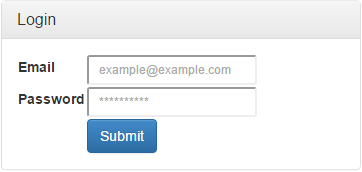
\includegraphics[width=0.5\textwidth]{img/zf2/login-container.png}
	\caption{Login container}
	\label{fig:login-container}
\end{figure}
	
	\subsection{Voucher system}

This system required operations with money and we come up with great solution, to implement voucher system. Customers have to buy vouchers to top up their balance on the account. Cards has to be printable and in order to do so I am generating a \textit{*.pdf} file that can be printed or saved for future printing. Voucher contains short information about company and \textit{QR code} that allow to scan by smartphone to simplify code inserting process. Figure \ref{fig:voucher} shows an example of printed voucher.

\begin{figure}[H]
	\centering
	
\includegraphics[width=0.5\textwidth]{img/zf2/voucher-example.png}
	\caption{Voucher example}
	\label{fig:voucher}
\end{figure}
	
To design this voucher and make it printable from web browser, I am using \textit{DOM pdf} generator. It allows to display remote pictures and specify fixed positions for text. \textit{QR Code} generating module submits the \textit{HTTP} request to Google API and receives a dynamic link to an image, which later in page generation I am using to add into \textit{pdf} file.


	\subsubsection{Lookup vouchers}
	

	\subsection{Order system}
		\subsubsection{Placed orders}
			When customer using their application places the order and transaction fully completed, then this order appears on the \textit{home page} as this system is designed to be pre order. At the certain time before collection system administrator prints out the list of food that has to be prepared for customer. In order to make a good printable layout it creates a \textit{*.pdf} file using \textit{JavaScript} module called PDF make ~\cite{PDF_Make_module}. It uses Document definition object and you do not have to calculate position manually as like in other pdf generation libraries. For example it can be as simple as:
			\\
			\begin{minted}{JavaScript}
var docDefinition = {
content: [
    // if you don't need styles, you can use a simple string to define a paragraph
    'This is a standard paragraph, using default style',

    // using a { text: '...' } object lets you set styling properties
    { text: 'This paragraph will have a bigger font', fontSize: 15 },

    // if you set pass an array instead of a string, you'll be able
    // to style any fragment individually
    {
      text: [
        'This paragraph is defined as an array of elements to make it possible to ',
        { text: 'restyle part of it and make it bigger ', fontSize: 15 },
        'than the rest.'
      ]
    }
  ]
};
			\end{minted}
			
			
			When you have prepared your document-definition-object, you can run the function that will parses it and generated \textit{pdf}:
			\\
			
			\begin{minted}{JavaScript}
// open the PDF in a new window
pdfMake.createPdf(docDefinition).open();
 
// print the PDF (temporarily Chrome-only)
pdfMake.createPdf(docDefinition).print();
 
// download the PDF (temporarily Chrome-only)
pdfMake.createPdf(docDefinition).download('optionalName.pdf');
			\end{minted}
			
			After order has been processed and collected, administrator has to go back to this system and mark collected orders. To simplify this process there is a check box beside each order and when all collected orders are marked user have to click \textit{Collected} button to make an update.
			\\
			In case of emergency some customer canceled their order administrator is allowed to cancel selected order and return money to customers account. In that case this order will not appear in later reports.
			
		\subsubsection{Order Reports}
			In order to make an accounting report in the orders tab, administrator can select two types of reports:
			\begin{itemize}
				\item \textbf{Daily report}
				\item \textbf{Periodic report}
			\end{itemize} 
			
			To view daily report user should specify the date in \textit{mm/dd/yyyy} format and press submit button as you can see in figuer \ref{fig:select-report-page}. 
			
			\begin{figure}[H]
				\centering
				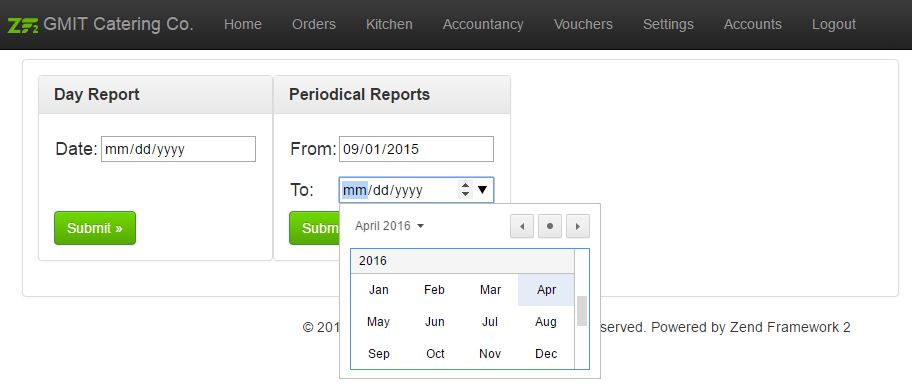
\includegraphics[width=1\textwidth]{img/zf2/01-canteen_select_periodic_report_page.png}
				\caption{Daily/Periodic report page}
				\label{fig:select-report-page}
			\end{figure}
			
			In the new page it will display report based on the period or specific date. Where user can go further and click order details, see customer's information or print this page as a report, see figure \ref{fig:daily-report-page}.
			
			\begin{figure}[H]
				\centering
				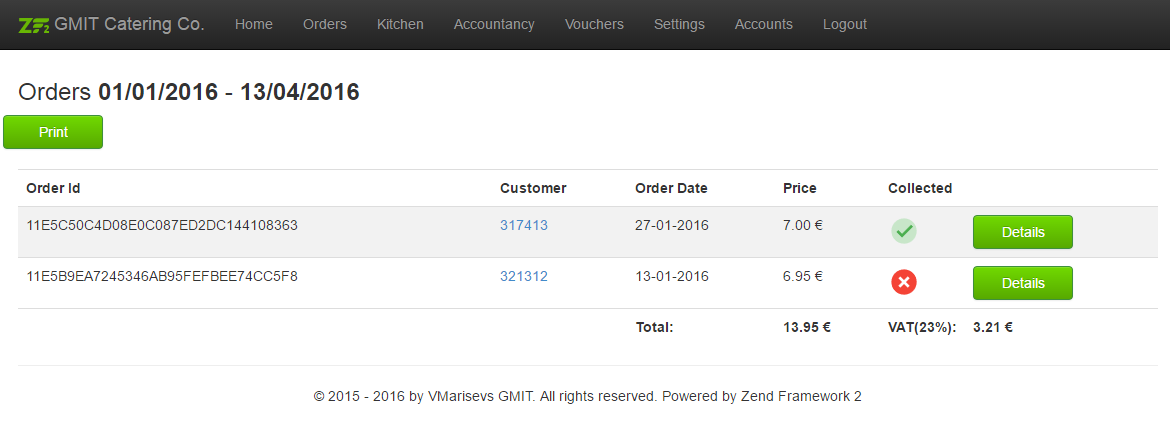
\includegraphics[width=1\textwidth]{img/zf2/01-canteen_select_periodic_report_page_1.png}
				\caption{Daily/Periodic report page}
				\label{fig:daily-report-page}
			\end{figure}
			
			Order details will display full information about customer and items ordered. It can be printed separately as invoice (see figure \ref{fig:order-invoice-page}) or proceed to go and view customer personal details.
			
			\begin{figure}[H]
				\centering
				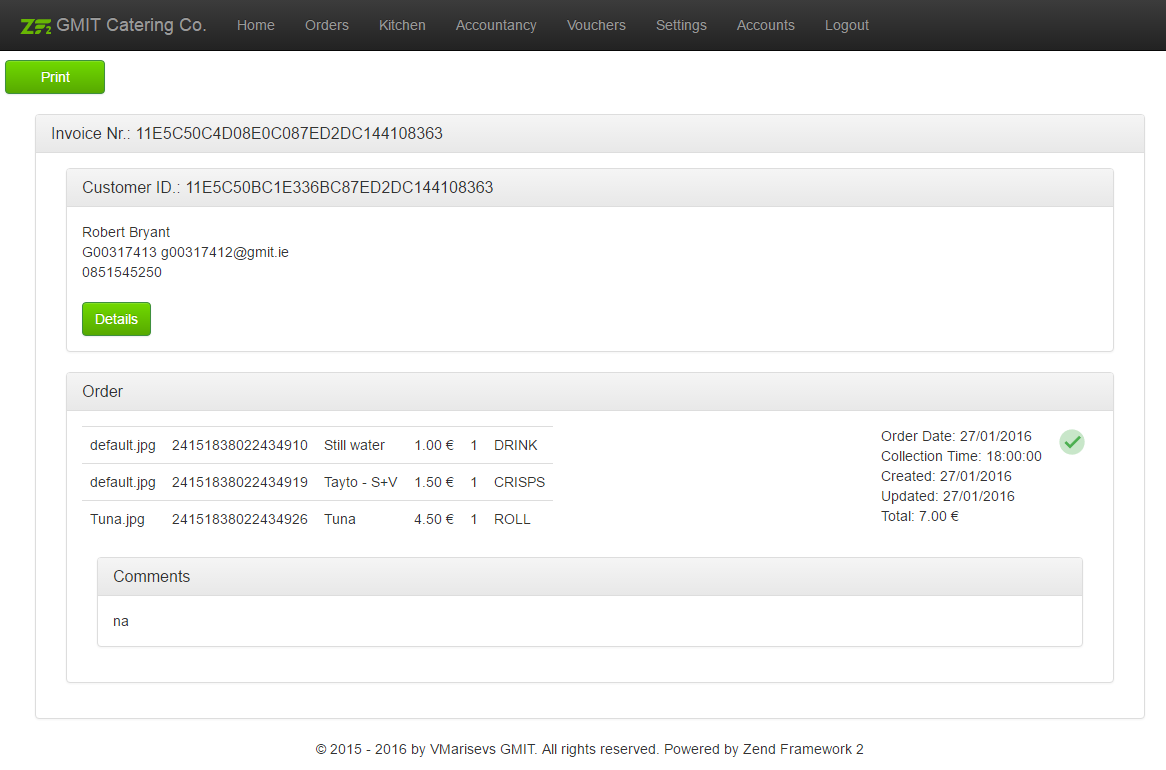
\includegraphics[width=1\textwidth]{img/zf2/01-canteen_select_periodic_report_page_2.png}
				\caption{Daily/Periodic report page}
				\label{fig:order-invoice-page}
			\end{figure}
			
			
		
		
		
	\subsection{Customer and accountancy}
		\subsubsection{Customer details}
		
		Authorized person can view all registered customers in accountancy tab and by clicking \textit{view} button. It will display a table with all users see in figure \ref{fig:customer-list}
		
		\begin{figure}[H]
			\centering
			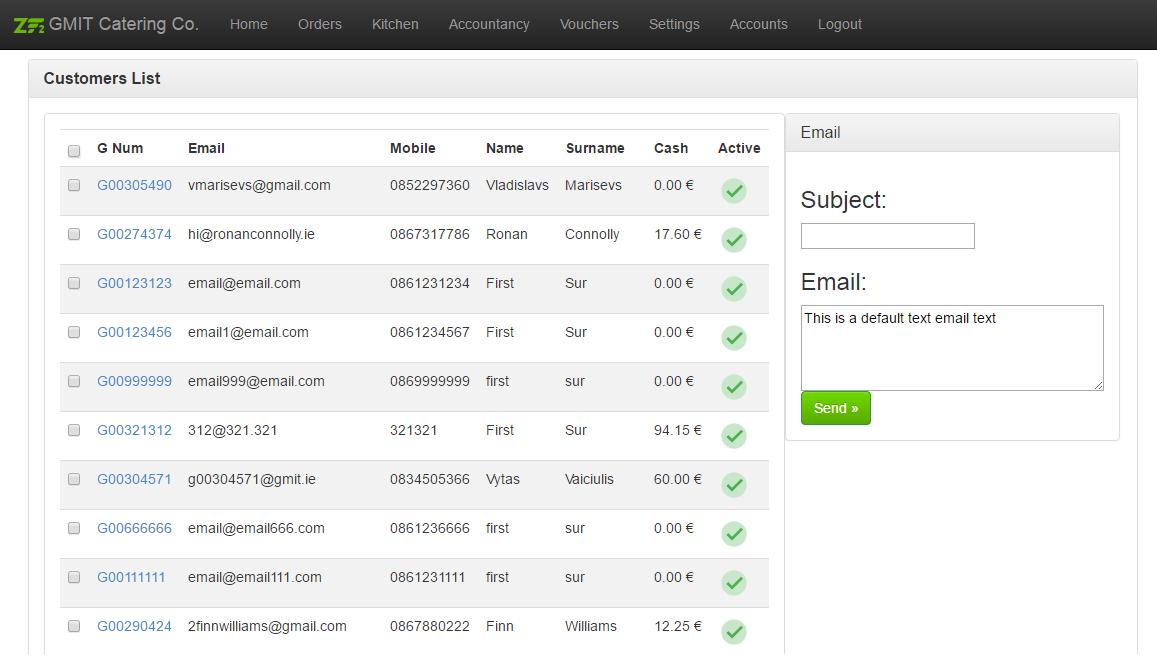
\includegraphics[width=1\textwidth]{img/zf2/04-customers.png}
			\caption{Customers list}
			\label{fig:customer-list}
		\end{figure}
		
		In this page we can select customers which we want to inform in updates and send them an email from default email. 
		% (This configuration was mentioned earlier in Database chapter)
		When person is found we can view his details as you can see in \ref{fig:customer-details} figure.
		
		\begin{figure}[H]
			\centering
			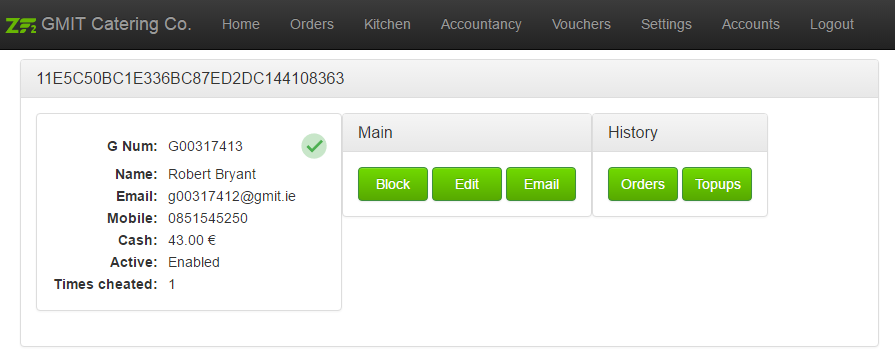
\includegraphics[width=1\textwidth]{img/zf2/02-customer_information.png}
			\caption{Customers details}
			\label{fig:customer-details}
		\end{figure}
		
		In this section we are able to do such things like send an email to customer, block him or edit his personal details in case they are wrong. We can determine that this cheated once, this counter increments only when person tries to enter wrong QR code as their voucher. 
		
		\subsubsection{Customer history}
		User has two types of histories. First one keeps a track of all user orders, so in future it can suggest user to make similar orders and history of user balance top up.
		
		
		\begin{figure}[H]
			\centering
			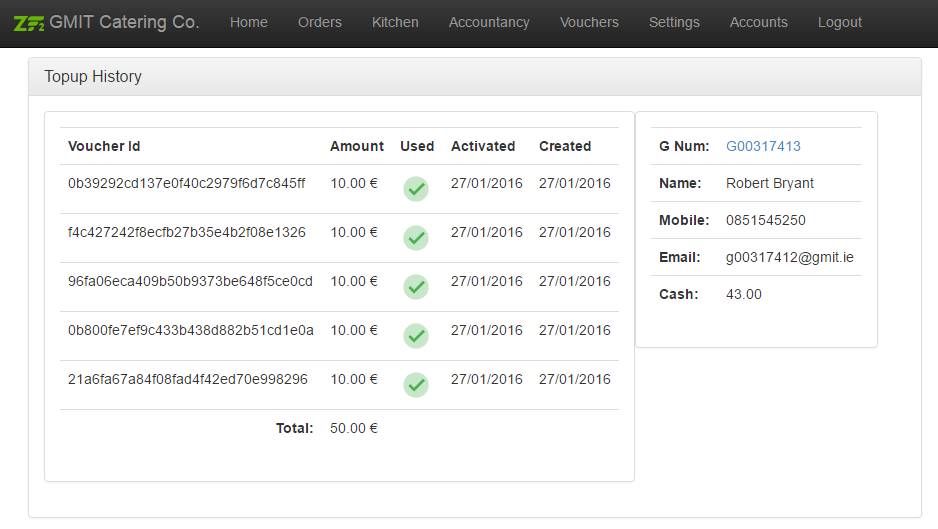
\includegraphics[width=1\textwidth]{img/zf2/02-customer_information_topup_history.png}
			\caption{Customers top up history}
			\label{fig:customer-topup-history}
		\end{figure}
		
		\begin{figure}[H]
			\centering
			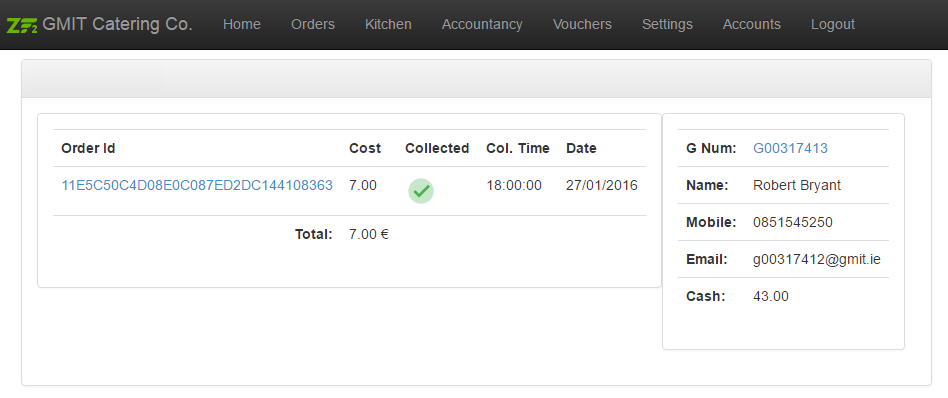
\includegraphics[width=1\textwidth]{img/zf2/02-customer_information_order_history.png}
			\caption{Customers order history}
			\label{fig:customer-order-history}
		\end{figure}
		
	\subsection{Ionic routes \& functions}
		In order to establish interconnection between Ionic and Zend Framework we are using JSON interface. To secure the routes that available for mobile application we added special paths on which API would response. When application queries the \textit{http://.../getfood/} it will return JSON type string with all food available. In order to deal with customers we have specialized roots for them, for example \textit{http://.../userhistory[/:customerID][/:customerPW]}. Using this path RDBMS will return complete user order history in JSON format. Note that the password is hashed on the Ionic side and passed just a hash code and user id. This sort of combination would be quite difficult to guess. We also have more routes that are designed using similar principle:
		\begin{itemize}
			\item *Authenticate customer
			\item *Recover customers password
			\item *Sign Up new customer
			\item *Top Up customer balance
			\item *Approve customer's order and purchase
			\item *Show customers history
			\item *Show available food
		\end{itemize}
	



\pagebreak
  \section{Mobile App}
Here we will go though all the different sections of the mobile application.
\\

There are three tabs in the application, Orders, About and Account.
These are located on the bottom for iOS and on the top for Android.
This gives a native experience, look and feel to the user.
\\

I will refer to each view as a page below.

\subsection{Sections}
A description of each part of the mobile application.
\\

% 1
\begin{minipage}{5cm}
	\begin{figure}[H]
		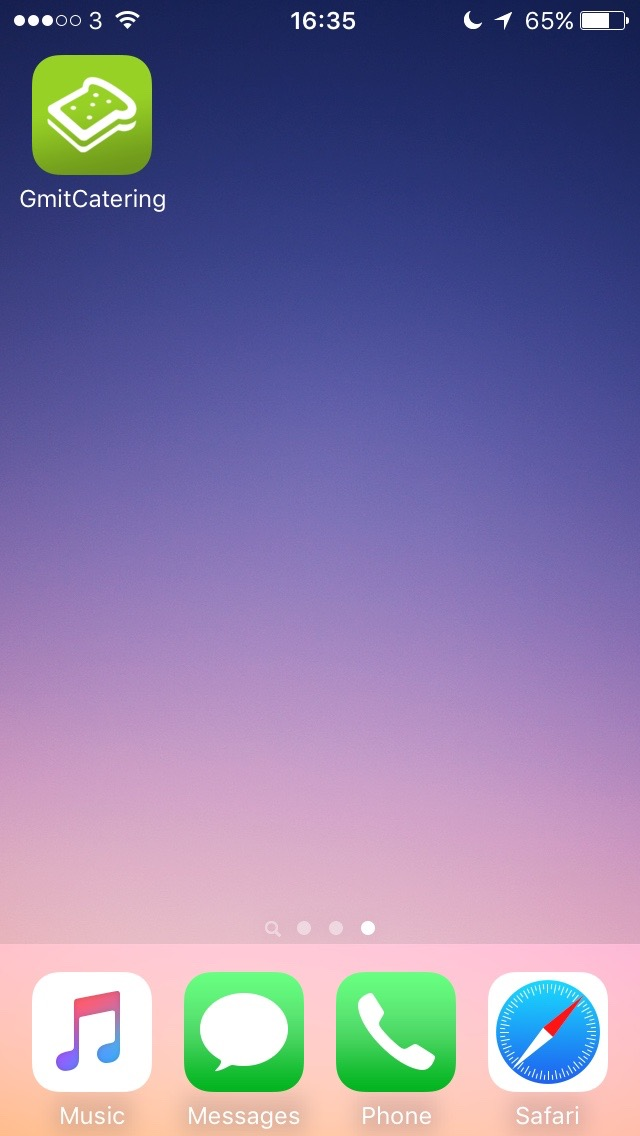
\includegraphics[width=5cm]{img/mobile-app/screen-shots/IMG_2903.jpg}
		\caption{Home Screen}
	\end{figure}
\end{minipage} \hfill
\begin{minipage}{0.55\textwidth}
We can see the application icon on the \textbf{home screen}.
\\

Initially we were going to try and incorporate the GMIT logo into the design but that seemed too tacky.
\\

We used the GMIT Catering green colour with a slight gradient, then overlaid a simple sandwich icon in white.
\end{minipage}

% 2
\begin{minipage}{0.55\textwidth}
The first screen you encounter after tapping on the application is the \textbf{splash screen}, which is just a larger version of the application icon.
You usually only see this the first time you open the application or if you are running on an older device.
\\

Once loaded you will see the \textbf{login} page, where we ask for your ID and Password.
This form contains validation and error messages above the input boxes.
You may only tap the \textbf{Sign In} button once the form is valid.
We have incorporated this into all forms in the application.
\\

Once logged in you will stay logged in, even after closing the application, you can log out from within the application.

You also have access to the \textbf{Sign Up} and \textbf{Reset Password} pages.
\end{minipage}
\begin{minipage}{5cm}
	\begin{figure}[H]
		\includegraphics[width=5cm]{img/mobile-app/screen-shots/IMG_2904.jpg}
		\caption{Login}
	\end{figure}
\end{minipage} \hfill


% 3
\begin{minipage}{5cm}
	\begin{figure}[H]
		\includegraphics[width=5cm]{img/mobile-app/screen-shots/IMG_2905.jpg}
		\caption{Password Reset}
	\end{figure}
\end{minipage} \hfill
\begin{minipage}{0.55\textwidth}
If you forget your password you can enter your ID and Email into this form, and a new password will be emailed to you.
\\

You can then edit your password from within the application later on.
\end{minipage}

% 4
\begin{minipage}{0.55\textwidth}
The \textbf{Sign Up} page contains a few basic instructions above the form, then some error messages, and finally the form itself.
\\

There is extra form validation here, such as regular expressions to make sure that all characters are valid, for instance only alpha characters are allowed in the name fields, no spaces or apostrophes. 
Once you sign up you will automatically be logged in.
\\

Password input on all forms are hashed with \textbf{MD5} instantly.
We may input any characters as the password will be hashed into valid characters.
It also means that there passwords are not stored in plain text, MD5 hashes cannot be un-hashed.
\\

We felt this was a necessary step for security and privacy purposes.
\end{minipage}
\begin{minipage}{5cm}
	\begin{figure}[H]
		\includegraphics[width=5cm]{img/mobile-app/screen-shots/IMG_2906.jpg}
		\caption{Sign Up}
	\end{figure}
\end{minipage} \hfill

% 5
\begin{minipage}{5cm}
	\begin{figure}[H]
		\includegraphics[width=5cm]{img/mobile-app/screen-shots/IMG_2907.jpg}
		\caption{Orders}
	\end{figure}
\end{minipage} \hfill
\begin{minipage}{0.55\textwidth}
From the \textbf{orders} page we can see all the sandwiches that are available.
\\

This data is taken from our web server and can be changed instantly.

\end{minipage}

% 6
\begin{minipage}{0.55\textwidth}
When we tap on a sandwich we our brought to the order page for that sandwich.
\\

We can view more information about the chosen sandwich from here.
\\

We must then choose a bread and order time.
\\

There are optional requirements such as: a drink, crisps, up to four miscellaneous items and a text comment.
The miscellaneous items mostly include add ons for the sandwich such as re onion, lettuce and things of that nature.

\end{minipage}
\begin{minipage}{5cm}
	\begin{figure}[H]
		\includegraphics[width=5cm]{img/mobile-app/screen-shots/IMG_2908.jpg}
		\caption{Order Details}
	\end{figure}
\end{minipage} \hfill

% 7
\begin{minipage}{5cm}
	\begin{figure}[H]
		\includegraphics[width=5cm]{img/mobile-app/screen-shots/IMG_2909.jpg}
		\caption{Order Details}
	\end{figure}
\end{minipage} \hfill
\begin{minipage}{0.55\textwidth}
At the bottom of the \textbf{order details} page we can see our current balance, the total cost for our order and a button to order it.
We can also see some details about order times.
\\

The \textbf{Order button} is only available during valid times and when we have sufficient balance.
\end{minipage}

% 8
\begin{minipage}{0.55\textwidth}
Once we press the \textbf{Order button} we are given a prompt showing us how much money we will have in our account after the order.
\\

This is important as the user may press the \textbf{Order button} by accident.
It also gives the user some time to go back and choose extra items.

\end{minipage}
\begin{minipage}{5cm}
	\begin{figure}[H]
		\includegraphics[width=5cm]{img/mobile-app/screen-shots/IMG_2910.jpg}
		\caption{Order Confirm}
	\end{figure}
\end{minipage} \hfill

% 9
\begin{minipage}{5cm}
	\begin{figure}[H]
		\includegraphics[width=5cm]{img/mobile-app/screen-shots/IMG_2911.jpg}
		\caption{Times}
	\end{figure}
\end{minipage} \hfill
\begin{minipage}{0.55\textwidth}
On the \textbf{About} page we can see today's opening times and order collection times.
\\

We can only order between opening times and may only choose to collect sandwiches at the order collection times allocated.
\end{minipage}

% 10
\begin{minipage}{0.55\textwidth}
Further down in the \textbf{About} page we can view information on the \textbf{Food Zone}, \textbf{Expresso Bar} and \textbf{Cafe Foyer}. 
\\

These are the three \textbf{GMIT Catering Company} locations throughout the college.
\end{minipage}
\begin{minipage}{5cm}
	\begin{figure}[H]
		\includegraphics[width=5cm]{img/mobile-app/screen-shots/IMG_2912.jpg}
		\caption{Espresso Bar}
	\end{figure}
\end{minipage} \hfill

% 11
\begin{minipage}{5cm}
	\begin{figure}[H]
		\includegraphics[width=5cm]{img/mobile-app/screen-shots/IMG_2913.jpg}
		\caption{Contact Us}
	\end{figure}
\end{minipage} \hfill
\begin{minipage}{0.55\textwidth}
At the very bottom of the \textbf{About} page we can see the \textbf{Contact Us} card.
\\

Which gives the user a simple way to email the \textbf{GMIT Catering Company} or to interact with them on Facebook.
\\

This will allow the company to gain more Facebook followers also.
\end{minipage}

% 12
\begin{minipage}{0.55\textwidth}
From the \textbf{Account} page we can see the users cash.
\\
We also have options to:
	\begin{itemize}
		\item Top Up (QR Reader)
		\item Log out
		\item View our information
		\item View our history
		\item Change our  password
	\end{itemize}

Grouping all these actions into the \textbf{Account} page keeps the UI clean and organised.

\end{minipage}
\begin{minipage}{5cm}
	\begin{figure}[H]
		\includegraphics[width=5cm]{img/mobile-app/screen-shots/IMG_2914.jpg}
		\caption{Account}
	\end{figure}
\end{minipage} \hfill

% 13
\begin{minipage}{5cm}
	\begin{figure}[H]
		\includegraphics[width=5cm]{img/mobile-app/screen-shots/IMG_2915.jpg}
		\caption{QR Reader}
	\end{figure}
\end{minipage} \hfill
\begin{minipage}{0.55\textwidth}
When you tap on \textbf{Top up} you are given the prompt to purchase a top-up card from the \textbf{GMIT Catering} checkout or else continue to scan your card.
\\

A QR reader opens up form within the application and you can scan your card.
\\

On completion you will be let known if the top-up went through successfully or not.
\\

You will then be brought to the User Information page where you can see your cash balance updated (or not).
\end{minipage}

% 14
\begin{minipage}{0.55\textwidth}
In the \textbf{User History} page you can view all past orders.
\\

You can also see if it was marked as collected.
\\

If the order was cancelled by the \textbf{GMIT Catering} staff it will also be marked as collected.
Collected basically means is has been dealt with by the staff.
\\

\end{minipage}
\begin{minipage}{5cm}
	\begin{figure}[H]
		\includegraphics[width=5cm]{img/mobile-app/screen-shots/IMG_2916.jpg}
		\caption{Order History}
	\end{figure}
\end{minipage} \hfill

% 15
\begin{minipage}{5cm}
	\begin{figure}[H]
		\includegraphics[width=5cm]{img/mobile-app/screen-shots/IMG_2917.jpg}
		\caption{User Information}
	\end{figure}
\end{minipage} \hfill
\begin{minipage}{0.55\textwidth}
From the \textbf{User Information} page we can see the users:
	\begin{itemize}
		\item Cash
		\item ID
		\item Name
		\item Phone
	\end{itemize}
This can easily be extended to show other information.
\end{minipage}

% 16
\begin{minipage}{0.55\textwidth}
From the \textbf{Change Password} page we can change our password.
\\

This is very useful for when we email the user a temporary password.
\\

As you can see we have full form validation here.

\end{minipage}
\begin{minipage}{5cm}
	\begin{figure}[H]
		\includegraphics[width=5cm]{img/mobile-app/screen-shots/IMG_2918.jpg}
		\caption{Change Password}
	\end{figure}
\end{minipage} \hfill
    
\subsection{Use Cases}
There are many use cases for this application.
\\

First of all it create awareness of the GMIT Catering Company brand within the college.
There is various information about the different areas within the college that the company runs.
\\

There are links to email and Facebook which lets the users interact with the company.
\\

Users can view opening times, which is often a reason why many students do not visit the canteen, due to not knowing it's open.
\\

With push notifications the company can get messages straight to the customer each day, giving various offers, deals and promotions.
\\

Users can pre-order food which is a very popular thing to do now a days, especially due to the fact that it can keep you structured and make sure you follow a certain eating habit, without the evils of hunger to persuade you into binging.
\\

On top of this, it allows customers to skip the queue and for the staff to prepare sandwiches during quite hours (but before rush hours).

\subsection{Code Snippets}
Here we will list some interesting code snippets from the mobile application.
\\

The Ionic/Angular markdown/code for the \textbf{Login} page.

This includes the form validation, which uses \textbf{ng-messages}.
\begin{minted}[breaklines]{html}
<ion-view view-title="gmit catering" hide-nav-bar="true" class="splash-page login-page">
    <ion-content>
        <div class="padding logo">
            <h1>gmit catering</h1>
        </div>
    
        <div>
            <!-- errors -->
            <ng-messages for="loginForm.$error" class="error-text">
            <ng-message when="required">Required field missing</ng-message>
            <ng-message when="minlength">Minimum Length not met</ng-message>
            <ng-message when="maxlength">Maximum Length not met</ng-message>
            </ng-messages>
        </div>
    
        <form name="loginForm" class="form" ng-submit="userLogin(loginForm, loginForm.username, loginForm.password)" novalidate>
            <div class="card">
                <div class="list">
                    <label class="item item-input">
                        <span class="input-label">ID:</span>
                        <input name="name" type="tel" ng-model="loginForm.username" placeholder="G/C Number" minlength="6" maxlength="8" required />
                    </label>
                    <label class="item item-input">
                        <span class="input-label">Password</span>
                        <input name="pass" type="password" ng-model="loginForm.password" placeholder="********" minlength="3" maxlength="20" required />
                    </label>
                </div>
            </div>
            
            <div class="padding-left padding-right">
                <input type="submit" value="Sign in" class="button button-block button-balanced" ng-disabled="loginForm.$invalid" />
            </div>
        </form>
    
        <div class="padding splash-links splash-margin">
            <a href="#/signup" class="a-no-style">Sign Up</a>
        </div>
        
        <div class="padding splash-links splash-margin">
            <a href="#/reset" class="a-no-style">Reset Password</a>
        </div>
    </ion-content>
</ion-view>
\end{minted}

Next we can see the \textbf{userLogin} function that the above form calls on, here we are inside the \textbf{Login Controller}.

If the form is valid then we pass the request onto the auth function in the User service, we also have some error messages.

We are using the \textbf{.then} functionality of the Angular service function User.auth to allow us to wait until the request has finished, this is a basic form of a promise.
\begin{minted}[breaklines]{js}
$scope.userLogin = function(form, name, password) {
    var username = parseInt(name, 10);
    var success;
    var login = 1;
    
    if (form.$valid) {
        User.auth(username, password, login).then(function() {
            if (User.session_id === 1) {
                $scope.showSuccess("Login"); // alert
                IServices.pushinit(); // push notify setup and save user
            } else {
                if (User.connectionError === true) {
                    console.log('User.connectionError === true: failed');
                } else {
                    $scope.showError("Username or Password Incorrect");
                }
            }
        }, function() {
            console.log('userLogin: failed');
        });
    }
};
\end{minted}

Below is the regular expression used for the name fields.

Only alpha characters are allowed, this is used in conjunction with ng-pattern in the html form.
\begin{minted}[breaklines]{js}
$scope.regex_name = '^[a-zA-Z]+$';
\end{minted}

\pagebreak
\subsection{Diagram}
The Ionic mobile application contains many folders and files, some for styling, structure and others for running tasks, downloading templates and building binaries.
\\

\noindent Here is a list of the directories within the home directory:
\begin{itemize}[noitemsep,nolistsep]
\item hooks
\item test
\item node\_modules
\item platforms
\item plugins
\item privacy-policy
\item resources
\item scss
\item typings
\item www
\end{itemize}
There are also around 20 files for various functions as described above.
The actual development happens within the \textbf{www} folder (www because we are working within a web view).
\\

\noindent Here is an illustration of the contents within the \textbf{www} folder:
% full page width
\begin{center}
    \makebox[\textwidth]{\includegraphics[width=\paperwidth]{img/mobile-app/diagram.png}}
\end{center}

\section{HTTP RESTful Route Requests}
% go through all the HTTP routes, with code snippets
A listing of all the routes, including request and response data.
The request data is any data that we give (either in the URL via ':' or in the body of the HTTP request) to the server.
The response data is data received from the server in response to our HTTP request (in JSON format or else error 404).
\\

First I will show you an example of how we do a HTTP request in Angular. Since the most common function we use is for authorising the user, we will show you that one:
\begin{minted}[breaklines]{js}
        o.auth = function(username, password, login) {
            var passwordMd5 = md5.createHash(password);
            
            if (login) {
                o.showLoading();
            }
            
            var postTo = SERVER.url + "verifyuser/" + username + "/" + passwordMd5;
            
            return $http({
                method: 'GET',
                url: postTo
            }).then(function successCallback(response) {
            if (response.data.hasOwnProperty('customer_id')) {
                o.setSession(username, passwordMd5, 1, response.data.customer_id, response.data.customer_name, response.data.customer_surname, response.data.customer_email, response.data.customer_mobile, response.data.customer_address, response.data.customer_cash);
            }
            
            if (login) {
                o.hideLoading();
            }
            o.connectionError = false;
            
        }, function errorCallback(response) {
        if (login) {
            o.hideLoading();
        }
        o.connectionError = true;
    });
};
\end{minted}
Here we can see we first hash the users password with MD5.
Then we show the loading animation/spinner, next we create the URL and make the HTTP request.
Once we have a response we save the data and hide the loading animation/spinner, or else show an error message.
\\

The rest of the HTTP requests follow a similar format.
\linebreak

\noindent We start the url with a prefix then add on the url function that we wish to use. \\

\textbf{Prefix:}
\begin{itemize}[noitemsep,nolistsep]
\item \textbf{Production:} \url{http://canteenapplication.vmarisevs.me/mobileapplication/}
\item \textbf{Development:} \url{https://catering-test-server.herokuapp.com/}
\end{itemize}
%code snippets?

Below I will show the URL structure, along with an example request and response.

\subsection*{Create User}
\textbf{URL:}
\begin{minted}[breaklines]{yaml}
createuser[/:customerLogin][/:customerPW][/:customerEmail][/:customerMobile] [/:customerName][/:customerSurname][/:customerAddress]
\end{minted}

\textbf{Request:}
\begin{minted}[breaklines]{yaml}
createuser/123123/pw/email@email.com/0861231234/First/Sur/address
\end{minted}

\textbf{Response:}
\begin{minted}[breaklines]{JSON}
{"customer_identifier":"11E578C39D1DAE2881B43FAA99013818"}
\end{minted}

\subsection*{Login/Verify User}
\textbf{URL:}
\begin{minted}[breaklines]{yaml}
verifyuser[/:customerLg][/:customerPW]
\end{minted}

\textbf{Request:}
\begin{minted}[breaklines]{yaml}
verifyuser/123123/pw
\end{minted}

\textbf{Response:}
\begin{minted}[breaklines]{JSON}
{"customer_id":"11E4E6370B663F0D81B9EC9A743CC2AE",
"customer_name":"Regina"
,"customer_surname":"Walsh",
"customer_cash":"10.20",
"customer_mobile":"0853243435"}
\end{minted}

\subsection*{Get Food}
\textbf{URL:}
\begin{minted}[breaklines]{yaml}
getfood
\end{minted}

\textbf{Request:}
\begin{minted}[breaklines]{yaml}
getfood
\end{minted}

\textbf{Response:}
\begin{minted}[breaklines]{JSON}
[{"food_id":"23961698511618135",
"food_name":"BLT", "food_description":"Grilled Bacon,\nSliced Tomato,\nCrisp Lettuce,\nMayonnaise\n","food_price":"3.95",
"food_type":"ROLL","food_picture":"BLT.jpg"}, {"food_id":"23961698511618136",
"food_name":"Baked Ham & Cheese", "food_description":"Baked Ham,\nMozzarella Cheese, \nCheddar Cheese,\nCountry Relish\n",
"food_price":"3.95", "food_type":"ROLL","food_picture":"BakedHamnCheese.jpg"}]
\end{minted}

\subsection*{User History}
\textbf{URL:}
\begin{minted}[breaklines]{yaml}
userhistory[/:customerID][/:customerPW]
\end{minted}

\textbf{Request:}
\begin{minted}[breaklines]{yaml}
userhistory/11E4E6370B663F0D81B9EC9A743CC2AE/pw
\end{minted}

\textbf{Response:}
\begin{minted}[breaklines]{JSON}
{"orders":{"11E55B538748A90AA04434E6D77FF0A4":{"order_collected":"0",
"order_comments":"\"some comment\"", "order_collection_time":"12:00:00",
"order_posted":"2015-09-15 02:42:50","food":[{"food_id":"23961698511618135",
"food_name":"BLT", "food_description":"Grilled Bacon,\nSliced Tomato,\nCrisp Lettuce,\nMayonnaise\n",
"food_price":"3.95","food_count":"1", "food_type":"ROLL","food_pic":"BLT.jpg"},{"food_id":"23961698511618141",
"food_name":"500ml still water","food_description":"","food_price":"1.00", "food_count":"1","food_type":"DRINK","food_pic":"default.jpg"}]}}}
\end{minted}

\subsection*{Change User Password}
\textbf{URL:}
\begin{minted}[breaklines]{yaml}
changeuserpw[/:customerID][/:customerPW][/:customerNewPW]
\end{minted}

\textbf{Request:}
\begin{minted}[breaklines]{yaml}
changeuserpw/11E55B29BCA900A6A04434E6D77FF0A4/pw/pww
\end{minted}

\textbf{Responses:}
\begin{minted}[breaklines]{JSON}
{"status":"OK"}

404
\end{minted}

\subsection*{Working Time}
\textbf{URL:}
\begin{minted}[breaklines]{yaml}
workingtime
\end{minted}

\textbf{Request:}
\begin{minted}[breaklines]{yaml}
workingtime
\end{minted}

\textbf{Response:}
\begin{minted}[breaklines]{JSON}
{"OrdersCollectionTime":["12:00:00","14:00:00"], "TodaysWorkingTime":{"open_time":null,"close_time":null}, "CurrentTime":"18:26:50"}
\end{minted}

\subsection*{Buy Food}
\textbf{URL:}
\begin{minted}[breaklines]{yaml}
buyfood[/:customerID][/:customerPW][/:collectionTime]
\end{minted}

\textbf{Request:}
\begin{minted}[breaklines]{yaml}
http://canteenapplication.vmarisevs.me/mobileapplication/buyfood/ 11E576B38F799E9281B43FAA99013818/pw/12:00?order_list= {%221%22:%2224151838022434887%22}&customer_comments=%22Hello%20Vlad%22
\end{minted}

\textbf{Responses:}
\begin{minted}[breaklines]{JSON}
{"status":"OK"}

404
\end{minted}

\subsection*{Recover User Password}
\textbf{URL:}
\begin{minted}[breaklines]{yaml}
recoveruserpw[/:customerLg][/:customerEmail]
\end{minted}

\textbf{Request:}
\begin{minted}[breaklines]{yaml}
recoveruserpw/305490/vmarisevs@gmail.com
\end{minted}

\textbf{Responses:}
\begin{minted}[breaklines]{JSON}
{"status":"OK"}

404
\end{minted}

\chapter{System Evaluation}	% n-m pages
\section{Management Website}
	\subsection{PDF make vs DOM PDF}
		One of most commonly used modules for generating \textit{pdf} is DOM PDF for Zend Framework 2. This module let you generate file based on html type content. It has advantages such as easy to install using \textit{composer}, interprets html page as structure of pdf file, loading pictures from remote sources. But it also has a big disadvantage to generate large file it will require more PHP hosting memory. 
		At the start all reports were planned to be made using DOM PDF module, but after testing, it show that there is not enough memory available for PHP services. 
		
		After doing some research on this problem, best solution was to increase RAM memory available for PHP service. On the local machine in the WAMP server you have to just change the \textit{memory\_limit} in the \textit{\textbf{php.ini}} file. That is a quick fix of this problem, but when it will come to upload this web application into real hosting, you will have same issue, because for increasing the  performance of your service you have to pay more money.
		
		To solve this problem and keep minimal required service performance, we decided to move pdf generation module from server side to client side. In this case website returns whole data that user required and it generates a report on the client computer. The idea was to use JavaScript that is interpreted by browser to create a pdf file \cite{PDF_Make_module}.
		
		Current web application uses both modules, domPDF is used for creating new vouchers. It generates maximum one page with 8 vouchers on it. They have specific margins for special paper and remotely created QR code to let users simply scan the code and top up their account balance. pdfMake can not be used for loading remote images, they have to be on the same origin. But when it comes to generate large list of invoices we are using a pdfMAKE that will send out the data to users computer and using JavaScript generates a pdf report that can be printed or saved.
	
\section{Mobile App}
\subsection{Chosen tech, why and how?}
% why and how we chose what
We chose to use Ionic because it is the most cutting edge cross platform technology out there at the moment.
It has the largest and most interactive developer community.
It seems like the obvious choice, even if JavaScript can be a pain in the neck.
\\

Angular and the web development tool-set was essential as that's what Ionic requires you to use, no choice here I'm afraid.
Steep learning curve but lots learned indeed.
\\

Heroku as a server was a joy to use.
iOS store was tricky but once learned not so bad.
Android store was simple and fun to learn.

\subsection{Alternatives tested}
% what other technologies did we test out?
Tested out Cordova, PhoneGap, JQueryMobile and Xamarin.
All were lacking in many areas.
\\

Again, Ionic was the clear winner.

\subsection{Robustness}
% is javascript/ionic robust?
JavaScript is lacking in robustness, this is inherent to the language itself.
Loose typing, implicit variable definitions and no real official guidelines or structure at all.
JavaScript doesn't even have a standard library.
\\

While this causes issues (there is not much error checking or auto-completion), you can get around it with plenty of console logging and getting comfortable with the Google Chrome Developer Tools.
Using transpiled languages like Microsoft's TypeScript gives more structure such as auto-completion and error checking.
\\

Google have done a good job at bringing structure to the JavaScript (and web development) world with the advent of Angular.
\\

We done much user testing in order to kink out any errors.
Something that unit tests may not find.

\subsection{Performance}
% is it performant compared to Android and Swift?
Ionic is as performant as we needed.
Our application contains various buttons, forms mixed with CSS and Animations.
There is not too much heavy duty calculation going on.
\\

Say if we were creating a game, or processing image data, then perhaps using Java(Android) or Swift would be something we'd have to look into.
\\

In regards to the structure of this project compared to Android and iOS, I think Angular does a good job at bringing structure to JavaScript.
The application is very modular and understandable (check out the diagram above to see how simple it is).

\subsection{Limitations}
\subsubsection{Native SDK Support}
% do we miss native sdk support?
With project Cordova we get access to most of the hardware available on the device, this still doesn't mean that we get access to Apples Kits (Health, Game, etc), but it does give us access to things like the TouchID sensor.

Some project may rely on the proprietary SDKs, but many project don't, and that's fine.

\subsubsection{Too new?}
% limitations of using such a new framework? breaks a lot?
We faced many issues while developing in the web development world, every day we had to update various dependencies.
If you haven't updated in a week, well you will be waiting a while before you start working.
\\

If a package decides to be removed from a repo, or a breaking change occurs on a package that one of your dependencies depends on.
Well prepare to navigate the GitHub issue tracker looking for others who have the same issue.
\\

If you have a large update, like for XCode, iOS or Ionic, then there may be a ripple effect.
\\

\textbf{Example:}
When I updated to iOS 8.2 on my iPhone, I tried to update my app through the Ionic command line tool, I get a strange error, so I run it with XCode, similar error, but I notice XCode needs to be updated as well. I go to update XCode, XCode states that there is an update for my Mac that needs to be installed.

The Mac OSX update takes an hour, XCode update takes an hour. Then once all finished I have to update Ionic.
Sometimes when updating XCode it removes the configuration file that you have set up previously, so you have to edit that.
\\

This is the kind of thing that happens with each major update and the first few times it is very confusing, but this is the world we live in, fast paced and never ending.

\chapter{Conclusion}	% 1-3 pages
% talk about the project as a whole

%what we learnt

%what we would do differently

%what we gained

%high level stuff

%last line should be quotable

%maybe quote somebody

\begin{comment}
\begin{itemize}
\item Briefly summarise your context and ob-jectives (a few lines).
\item Highlight your findings from the evalua-tion section / chapter and any opportuni-ties identified.
\end{itemize}
\end{comment}
